\documentclass[10pt]{beamer}\usepackage[]{graphicx}\usepackage[]{color}
% maxwidth is the original width if it is less than linewidth
% otherwise use linewidth (to make sure the graphics do not exceed the margin)
\makeatletter
\def\maxwidth{ %
  \ifdim\Gin@nat@width>\linewidth
    \linewidth
  \else
    \Gin@nat@width
  \fi
}
\makeatother

\definecolor{fgcolor}{rgb}{0.345, 0.345, 0.345}
\newcommand{\hlnum}[1]{\textcolor[rgb]{0.686,0.059,0.569}{#1}}%
\newcommand{\hlstr}[1]{\textcolor[rgb]{0.192,0.494,0.8}{#1}}%
\newcommand{\hlcom}[1]{\textcolor[rgb]{0.678,0.584,0.686}{\textit{#1}}}%
\newcommand{\hlopt}[1]{\textcolor[rgb]{0,0,0}{#1}}%
\newcommand{\hlstd}[1]{\textcolor[rgb]{0.345,0.345,0.345}{#1}}%
\newcommand{\hlkwa}[1]{\textcolor[rgb]{0.161,0.373,0.58}{\textbf{#1}}}%
\newcommand{\hlkwb}[1]{\textcolor[rgb]{0.69,0.353,0.396}{#1}}%
\newcommand{\hlkwc}[1]{\textcolor[rgb]{0.333,0.667,0.333}{#1}}%
\newcommand{\hlkwd}[1]{\textcolor[rgb]{0.737,0.353,0.396}{\textbf{#1}}}%
\let\hlipl\hlkwb

\usepackage{framed}
\makeatletter
\newenvironment{kframe}{%
 \def\at@end@of@kframe{}%
 \ifinner\ifhmode%
  \def\at@end@of@kframe{\end{minipage}}%
  \begin{minipage}{\columnwidth}%
 \fi\fi%
 \def\FrameCommand##1{\hskip\@totalleftmargin \hskip-\fboxsep
 \colorbox{shadecolor}{##1}\hskip-\fboxsep
     % There is no \\@totalrightmargin, so:
     \hskip-\linewidth \hskip-\@totalleftmargin \hskip\columnwidth}%
 \MakeFramed {\advance\hsize-\width
   \@totalleftmargin\z@ \linewidth\hsize
   \@setminipage}}%
 {\par\unskip\endMakeFramed%
 \at@end@of@kframe}
\makeatother

\definecolor{shadecolor}{rgb}{.97, .97, .97}
\definecolor{messagecolor}{rgb}{0, 0, 0}
\definecolor{warningcolor}{rgb}{1, 0, 1}
\definecolor{errorcolor}{rgb}{1, 0, 0}
\newenvironment{knitrout}{}{} % an empty environment to be redefined in TeX

\usepackage{alltt}


%\input{slides_header.tex}
\input{/home/sahir/git_repositories/epib607/inst/slides/slides_header2.tex}
\graphicspath{{/home/sahir/git_repositories/epib607/inst/slides/figure/}}


\newcommand{\Var}{\operatorname{Var}}
\newcommand{\Expec}{\operatorname{E}}
\newcommand{\Prob}{\operatorname{P}}

%\let\oldShaded\Shaded
%\let\endoldShaded\endShaded
%\renewenvironment{Shaded}{\footnotesize\oldShaded}{\endoldShaded}

%\newcommand{\blue}[1]{\textcolor{blue}{#1}}
%\newcommand{\red}[1]{\textcolor{red}{#1}}


\usepackage{xparse}
\NewDocumentCommand\mylist{>{\SplitList{;}}m}
{
	\begin{itemize}
		\ProcessList{#1}{ \insertitem }
	\end{itemize}
}
\NewDocumentCommand\mynum{>{\SplitList{;}}m}
{
	\begin{enumerate}
		\ProcessList{#1}{ \insertitem }
	\end{enumerate}
}
\newcommand\insertitem[1]{\item #1}

\newcommand\FrameText[1]{%
	\begin{textblock*}{\paperwidth}(0pt,\textheight)
		\raggedright #1\hspace{.5em}
\end{textblock*}}
\IfFileExists{upquote.sty}{\usepackage{upquote}}{}
\begin{document}
	
	
	



	\title{027 - Final Review}
\author{EPIB 607}
\institute{
	Sahir Rai Bhatnagar\\
	Department of Epidemiology, Biostatistics, and Occupational Health\\
	McGill University\\
	
	\vspace{0.1 in}
	
	\texttt{sahir.bhatnagar@mcgill.ca}\\
	%\texttt{\url{https://sahirbhatnagar.com/EPIB607/}}
}

\date{slides compiled on \today}

\maketitle



%\begin{frame}[label=toc]{Table of Contents}
%	\tableofcontents
%\end{frame}

%\AddButton

\section{Exam Details}
\begin{frame}{Exam Details}
	\small
		\begin{itemize}
	%	\setlength\itemsep{.51em}
		\item \textbf{When:} December 9, 2021. The exam will be made available on Crowdmark as of 9am EST for 24 hours. 
		\item This is a timed assessment. As soon as you download the exam, you will have 6 hours to complete and upload your solutions to Crowdmark. 
		\item \textbf{There will be a 5\% per hour lateness penalty.} Submissions by e-mail will not be accepted.
		\item This is an open book exam. Any material on myCourses (EPIB607/613) and personal notes are permitted.
		\item You are not permitted to use the internet and you must work alone. Using the internet or obtaining help from anyone else is considered Cheating as per \href{https://www.mcgill.ca/students/srr/academicrights/integrity/cheating}{Article 17 of the Code of Student Conduct and Disciplinary Procedures}
%	\item The exam is out of 70. There are 7 questions, each worth 10 points. Write down all your answers in the provided booklet. 
		\item Provide units and state your assumptions when applicable. Label axes and write answers in complete sentences when appropriate.
		\item The format of the exam will follow the assignments and the midterm. That is, you will be required to complete a series of questions in an RMarkdown document and knit to pdf. Your solutions for each question must then be uploaded to Crowdmark. A template will be provided which will also include the questions. 
		%\item There will be no live zoom meeting. You can email me should you have questions. 
		%\item Some commonly used $z$ and $t$ quantiles will be provided in a Table. If a question requires the use of $z$ or $t$ probabilites/quantiles not found in the provided Table, write the corresponding R code instead. When possible, you should complete the calculations.		
	\end{itemize}
	
\end{frame}

\begin{frame}{Topics to be covered}
	
	\textbf{Note that the exam is cumulative}
	
	\begin{enumerate}
		\setlength\itemsep{.51em}
		\item Data visualization (histograms, boxplots, scatterplots, line plots), Tidy Data, Color Palettes, grammar of graphics
		\item Descriptive statistics (mean, median, range, IQR, sd, correlation)
		\item Normal Curve Calculations, Sampling Distributions, CLT, Bootstrap
		\item Confidence intervals, Hypothesis Testing, p-values 
		\item One sample mean, one sample proportion, one sample rate
		\item Power and Sample size calculations
		\item Gaussian, Poisson, Binomial regression
		\item Permutation testing
		\item $\chi^2$ goodness of fit and ROC curves
	\end{enumerate}
	
\end{frame}

\section{Part I}

\section{Data visualization}

\begin{frame}{Aesthetics}
	\begin{itemize}
		\setlength\itemsep{.51em}
		\item Aesthetics
		\framedgraphic{scales.jpg}
		\pause 
		\item Commonly used aesthetics in data visualization: position, shape, size, color, line width, line type. Some of these aesthetics can represent both continuous and discrete data (position, size, line width, color) while others can only represent discrete data (shape, line type)	
	\end{itemize}
\end{frame}

\begin{frame}{Types of Graphs}
	\begin{itemize}
		\item Review the types of graphs created in the assignments.
		\item You should be able to critique a graph and propose appropriate graphics for a given dataset. Be mindful of the research question. The graphic should try to answer the research question. 
		\item \url{https://serialmentor.com/dataviz/directory-of-visualizations.html}
		\item \url{https://www.data-to-viz.com/}
	\end{itemize}
\end{frame}

\begin{frame}{How many scales are being used?}
	\centering
	\includegraphics[scale=0.4]{005-7.png}
\end{frame}


\begin{frame}[fragile]{Boxplots with qualitative palette}
\begin{knitrout}\tiny
\definecolor{shadecolor}{rgb}{0.969, 0.969, 0.969}\color{fgcolor}\begin{kframe}
\begin{alltt}
\hlkwd{library}\hlstd{(oibiostat);} \hlkwd{data}\hlstd{(}\hlstr{"famuss"}\hlstd{)}
\hlkwd{library}\hlstd{(ggplot2)}
\hlkwd{library}\hlstd{(colorspace)}

\hlkwd{ggplot}\hlstd{(famuss,} \hlkwd{aes}\hlstd{(}\hlkwc{x} \hlstd{= actn3.r577x,} \hlkwc{y} \hlstd{= bmi,} \hlkwc{fill} \hlstd{= actn3.r577x))} \hlopt{+}
\hlkwd{geom_boxplot}\hlstd{()} \hlopt{+}
\hlstd{colorspace}\hlopt{::}\hlkwd{scale_fill_discrete_qualitative}\hlstd{()}
\end{alltt}
\end{kframe}

{\centering 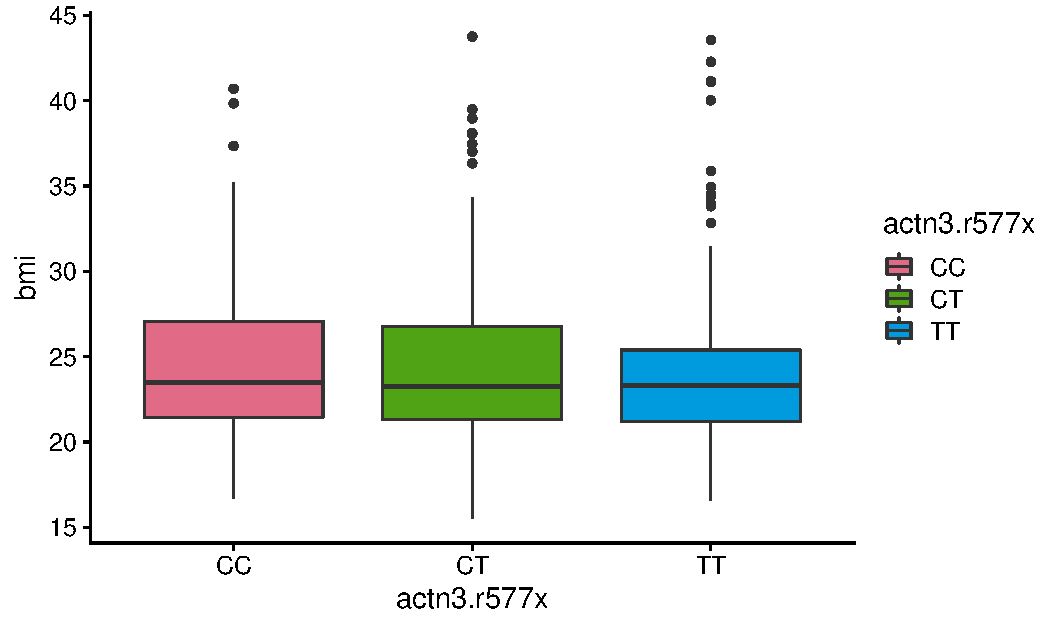
\includegraphics[width=\maxwidth]{figure/unnamed-chunk-2-1} 

}


\end{knitrout}
\end{frame}


\begin{frame}[fragile]{Conditional distribution of genotype \textit{given} race}
\begin{knitrout}\tiny
\definecolor{shadecolor}{rgb}{0.969, 0.969, 0.969}\color{fgcolor}\begin{kframe}
\begin{alltt}
\hlstd{sjPlot}\hlopt{::}\hlkwd{plot_xtab}\hlstd{(famuss}\hlopt{$}\hlstd{race, famuss}\hlopt{$}\hlstd{actn3.r577x,} \hlkwc{margin} \hlstd{=} \hlstr{"row"}\hlstd{)}
\end{alltt}
\end{kframe}

{\centering 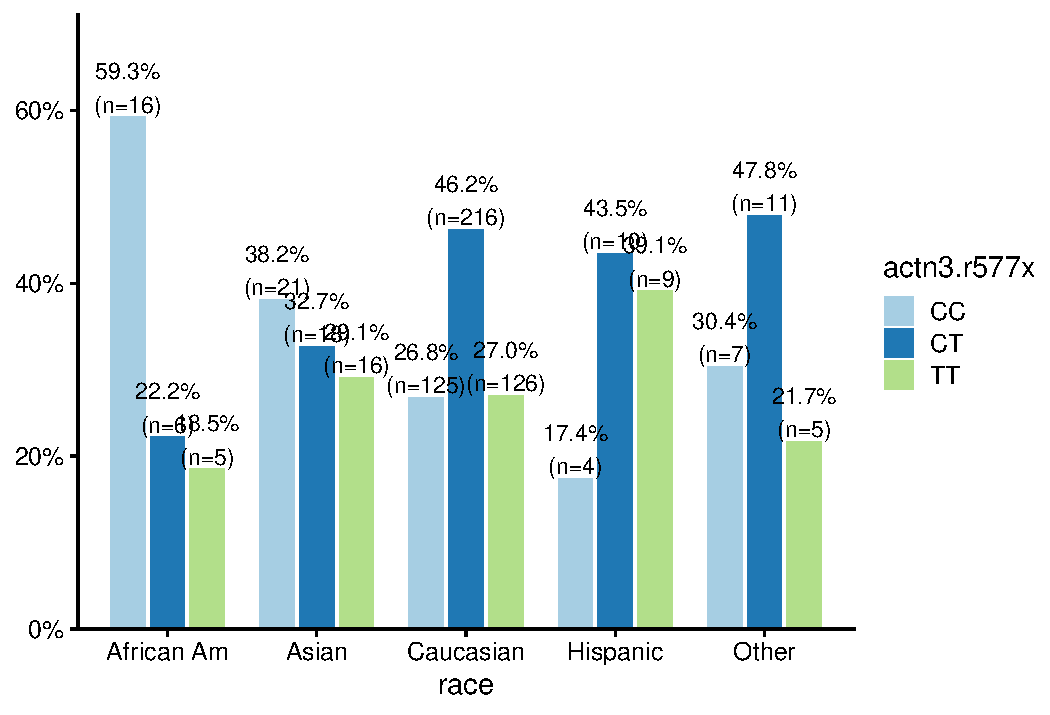
\includegraphics[width=\maxwidth]{figure/unnamed-chunk-3-1} 

}


\end{knitrout}
\end{frame}





\begin{frame}[fragile]{Scatter plots with sequential palette}
\begin{knitrout}\tiny
\definecolor{shadecolor}{rgb}{0.969, 0.969, 0.969}\color{fgcolor}\begin{kframe}
\begin{alltt}
\hlkwd{ggplot}\hlstd{(famuss,} \hlkwd{aes}\hlstd{(}\hlkwc{x} \hlstd{= height,} \hlkwc{y} \hlstd{= weight,} \hlkwc{color} \hlstd{= bmi))} \hlopt{+}
\hlkwd{geom_point}\hlstd{()} \hlopt{+}
\hlstd{colorspace}\hlopt{::}\hlkwd{scale_color_continuous_sequential}\hlstd{(}\hlkwc{palette} \hlstd{=} \hlstr{"Viridis"}\hlstd{)}
\end{alltt}
\end{kframe}

{\centering 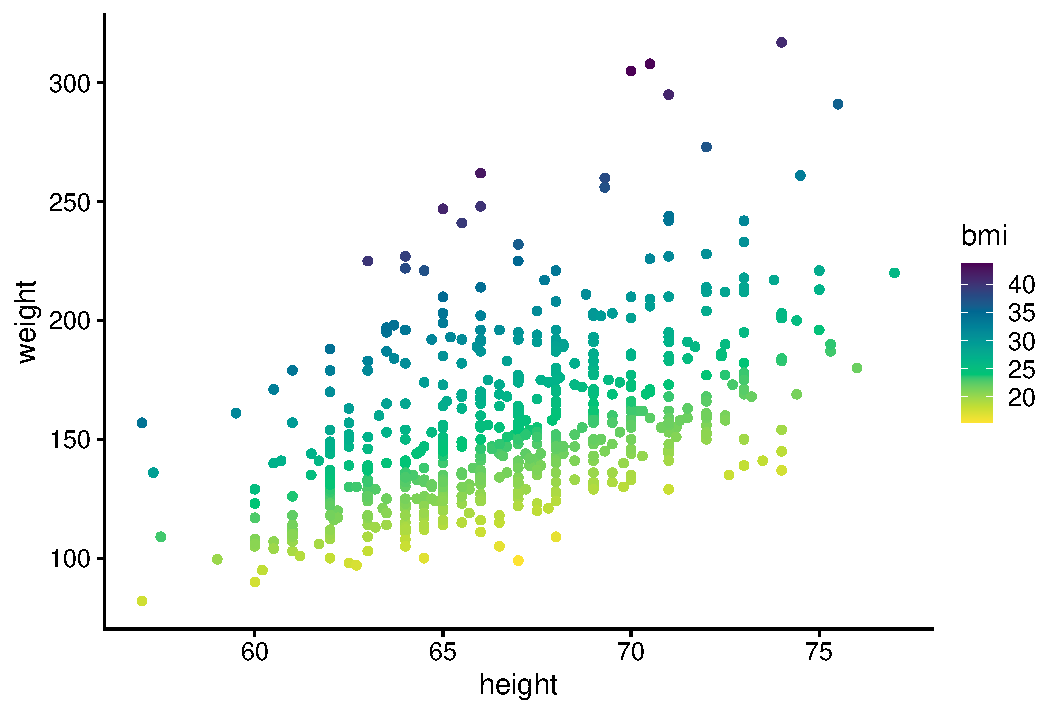
\includegraphics[width=\maxwidth]{figure/unnamed-chunk-4-1} 

}


\end{knitrout}
\end{frame}



\begin{frame}{Variable Types}
	\begin{itemize}
		\setlength\itemsep{1.5em}
		\item quantitative/numerical continuous (1.3, 5.7, 83, $1.5\times 10^{-2}$)
		\item quantitative/numerical discrete (1,2,3,4)
		\item qualitative/categorical unordered (dog, cat, fish)
		\item qualitative/categorical ordered (good, fair, poor)
	\end{itemize}
	
	
	
\end{frame}




\begin{frame}[fragile]{Color Palettes: Cynthia Brewer}
	
\begin{knitrout}\tiny
\definecolor{shadecolor}{rgb}{0.969, 0.969, 0.969}\color{fgcolor}\begin{kframe}
\begin{alltt}
\hlstd{pacman}\hlopt{::}\hlkwd{p_load}\hlstd{(RColorBrewer)}
\hlstd{RColorBrewer}\hlopt{::}\hlkwd{display.brewer.all}\hlstd{()}
\end{alltt}
\end{kframe}

{\centering 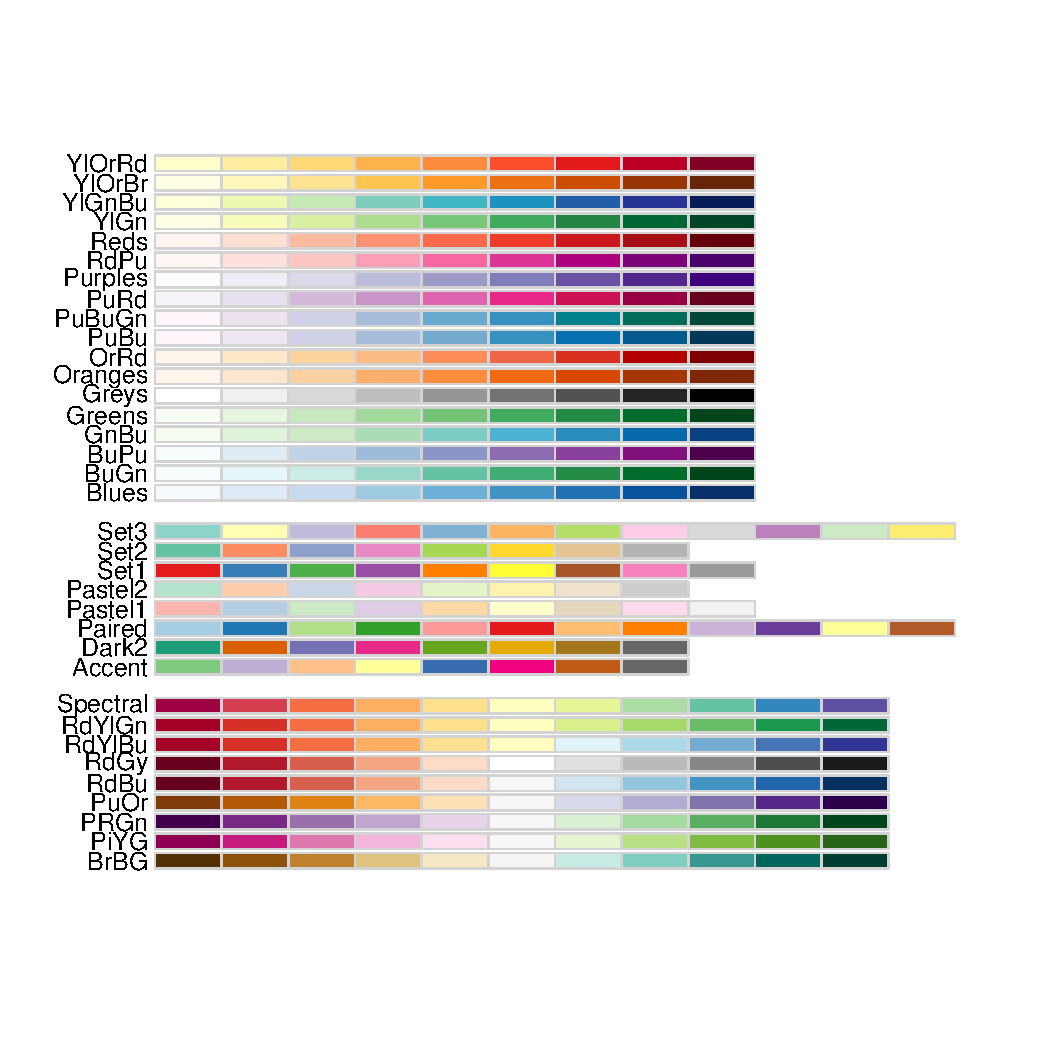
\includegraphics[width=\maxwidth]{figure/unnamed-chunk-5-1} 

}


\end{knitrout}
	
	
\end{frame}



\begin{frame}[fragile]{Color Palettes: viridis}
	
	
	
	\framedgraphic{viridis.png}
	
	
\end{frame}

\section{Tidy Data}

\begin{frame}{Tidy data}
	
	\begin{itemize}
		\setlength\itemsep{.51em}
		\item Each variable forms a column.
		\item Each observation forms a row.
		\item Each type of observational units forms a table
		\item Tidy data is ready for regression routines and plotting
	\end{itemize}
	
	
	\framedgraphic{tidy.png}
	
\end{frame}



\begin{frame}[fragile]{Example: Does a full moon affect behaviour?}
	
	\small
	\begin{itemize}
		\item Many people believe that the moon influences the actions of some individuals. 
		\item A study of dementia patients in nursing homes recorded various types of disruptive behaviors every day for 12 weeks. 
		\item Days were classified as moon days if they were in a 3-day period centered at the day of the full moon. 
		\item For each patient, the average number of disruptive behaviors was computed for moon days and for all otherdays. 
	\end{itemize}
	
\begin{knitrout}\footnotesize
\definecolor{shadecolor}{rgb}{0.969, 0.969, 0.969}\color{fgcolor}
\begin{tabular}{r|r|r}
\hline
patient & moon\_days & other\_days\\
\hline
1 & 3.33 & 0.27\\
\hline
2 & 3.67 & 0.59\\
\hline
3 & 2.67 & 0.32\\
\hline
4 & 3.33 & 0.19\\
\hline
5 & 3.33 & 1.26\\
\hline
6 & 3.67 & 0.11\\
\hline
7 & 4.67 & 0.30\\
\hline
\end{tabular}

\end{knitrout}
	
	
	
\end{frame}


\begin{frame}[fragile]{Not tidy vs. tidy data}
	
	
	%\Wider[4em]{
	%\centering
	
	\includegraphics[scale=0.45]{001-tidy3.pdf}
	
	
	%\framedgraphiccaption{tidy-fullmoon.jpg}{\texttt{text}}
	%}
	
\end{frame}

\begin{frame}[fragile]{Not tidy vs. tidy data}
	
	
	%\Wider[4em]{
	%\centering
	
	\includegraphics[scale=0.45]{001-tidy4.pdf}
	
	
	%\framedgraphiccaption{tidy-fullmoon.jpg}{\texttt{text}}
	%}
	
\end{frame}


\begin{frame}[fragile]{\texttt{tidyr::pivot\_longer()}}
	
	
	%\Wider[4em]{
	%\centering
	
	\includegraphics[scale=0.45]{001-tidy1.pdf}
	
	%\pause
	
\begin{knitrout}\tiny
\definecolor{shadecolor}{rgb}{0.969, 0.969, 0.969}\color{fgcolor}\begin{kframe}
\begin{alltt}
\hlstd{tidyr}\hlopt{::}\hlkwd{pivot_longer}\hlstd{(}\hlkwc{data} \hlstd{= df,} \hlkwc{cols} \hlstd{=} \hlopt{-}\hlstd{patient,} \hlkwc{names_to} \hlstd{=} \hlstr{"day_type"}\hlstd{,} \hlkwc{values_to} \hlstd{=} \hlstr{"mean_behavior"}\hlstd{)}
\end{alltt}
\end{kframe}
\end{knitrout}
	
	%\framedgraphiccaption{tidy-fullmoon.jpg}{\texttt{text}}
	%}
	
\end{frame}




\begin{frame}[fragile]{Plotting with tidy data}
	

	
\begin{knitrout}\tiny
\definecolor{shadecolor}{rgb}{0.969, 0.969, 0.969}\color{fgcolor}\begin{kframe}
\begin{alltt}
\hlkwd{ggplot}\hlstd{(}\hlkwc{data} \hlstd{= df_tidy,} \hlkwc{mapping} \hlstd{=} \hlkwd{aes}\hlstd{(}\hlkwc{x} \hlstd{= day_type,} \hlkwc{y} \hlstd{= mean_behavior,} \hlkwc{group} \hlstd{= patient))} \hlopt{+} \hlkwd{geom_line}\hlstd{()}
\end{alltt}
\end{kframe}
\end{knitrout}
	
\begin{knitrout}\tiny
\definecolor{shadecolor}{rgb}{0.969, 0.969, 0.969}\color{fgcolor}

{\centering 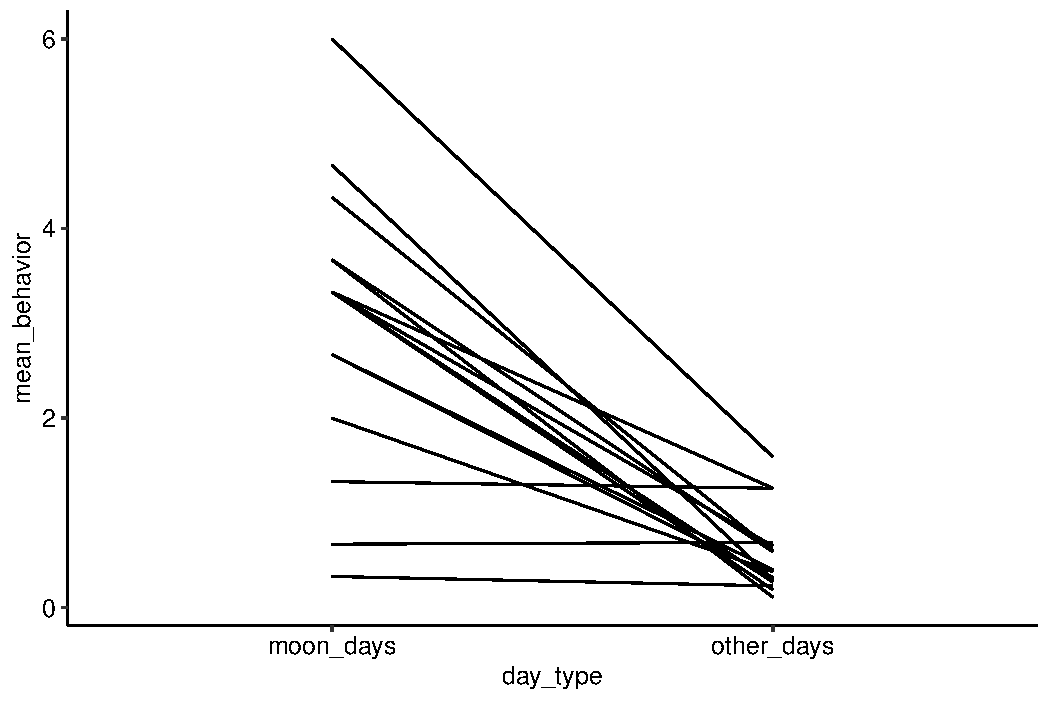
\includegraphics[width=\maxwidth]{figure/unnamed-chunk-10-1} 

}


\end{knitrout}
	
	
\end{frame}



\begin{frame}[fragile]{Regression with tidy data}
	
	
\begin{knitrout}\tiny
\definecolor{shadecolor}{rgb}{0.969, 0.969, 0.969}\color{fgcolor}\begin{kframe}
\begin{alltt}
\hlstd{fit} \hlkwb{<-} \hlstd{lme4}\hlopt{::}\hlkwd{lmer}\hlstd{(mean_behavior} \hlopt{~} \hlstd{day_type} \hlopt{+} \hlstd{(}\hlnum{1}\hlopt{|}\hlstd{patient),} \hlkwc{data} \hlstd{= df_tidy)}
\hlkwd{summary}\hlstd{(fit)}
\end{alltt}
\begin{verbatim}
## Linear mixed model fit by REML ['lmerMod']
## Formula: mean_behavior ~ day_type + (1 | patient)
##    Data: df_tidy
## 
## REML criterion at convergence: 90.3
## 
## Scaled residuals: 
##     Min      1Q  Median      3Q     Max 
## -2.2728 -0.3014 -0.0408  0.4860  2.4482 
## 
## Random effects:
##  Groups   Name        Variance Std.Dev.
##  patient  (Intercept) 0.1559   0.3948  
##  Residual             1.0663   1.0326  
## Number of obs: 30, groups:  patient, 15
## 
## Fixed effects:
##                    Estimate Std. Error t value
## (Intercept)          3.0220     0.2854  10.587
## day_typeother_days  -2.4327     0.3771  -6.452
## 
## Correlation of Fixed Effects:
##             (Intr)
## dy_typthr_d -0.660
\end{verbatim}
\end{kframe}
\end{knitrout}
\end{frame}














\begin{frame}[fragile]{Example: Is it tidy?}
	
	\centering
	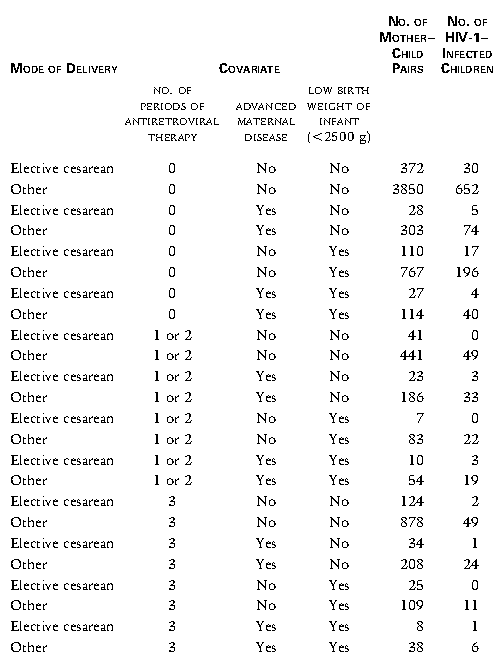
\includegraphics[scale=0.8]{hivtable.pdf}
	
	
\end{frame}


\section{Descriptive statistics}


\begin{frame}{Descriptive statistics}
	\begin{itemize}
		\setlength\itemsep{1.5em}
		\item Boxplots, histograms, density plot
		\item IQR, median, mode, mean, min, max, range
		\item Q1, Q3
		\item Skewness (long left/right tail)
		\item Correlation
	\end{itemize}
\end{frame}

\begin{frame}[fragile]{Descriptive stats by group}
\begin{knitrout}\small
\definecolor{shadecolor}{rgb}{0.969, 0.969, 0.969}\color{fgcolor}\begin{kframe}
\begin{alltt}
\hlkwd{library}\hlstd{(oibiostat);} \hlkwd{data}\hlstd{(}\hlstr{"famuss"}\hlstd{)}
\hlkwd{library}\hlstd{(dplyr)}

\hlstd{famuss} \hlopt
\hlstd{dplyr}\hlopt{::}\hlkwd{group_by}\hlstd{(actn3.r577x)} \hlopt
\hlstd{dplyr}\hlopt{::}\hlkwd{summarise}\hlstd{(}\hlkwc{mean_bmi} \hlstd{=} \hlkwd{mean}\hlstd{(bmi),}
\hlkwc{sd_bmi} \hlstd{=} \hlkwd{sd}\hlstd{(bmi))}
\end{alltt}
\begin{verbatim}
## # A tibble: 3 x 3
##   actn3.r577x mean_bmi sd_bmi
##   <fct>          <dbl>  <dbl>
## 1 CC              24.5   4.41
## 2 CT              24.5   4.55
## 3 TT              24.2   4.81
\end{verbatim}
\end{kframe}
\end{knitrout}
	
\end{frame}


\begin{frame}[fragile]{Subsetting data}
\begin{knitrout}\scriptsize
\definecolor{shadecolor}{rgb}{0.969, 0.969, 0.969}\color{fgcolor}\begin{kframe}
\begin{alltt}
\hlkwd{library}\hlstd{(oibiostat);} \hlkwd{data}\hlstd{(}\hlstr{"famuss"}\hlstd{)}
\hlkwd{library}\hlstd{(dplyr)}

\hlstd{f.male} \hlkwb{<-} \hlstd{famuss} \hlopt
\hlstd{dplyr}\hlopt{::}\hlkwd{filter}\hlstd{(sex} \hlopt{==} \hlstr{"Male"}\hlstd{)}


\hlstd{f.male.cauc} \hlkwb{<-} \hlstd{famuss} \hlopt
\hlstd{dplyr}\hlopt{::}\hlkwd{filter}\hlstd{(sex} \hlopt{==} \hlstr{"Male"} \hlopt{&} \hlstd{race} \hlopt{==} \hlstr{"Caucasian"}\hlstd{)}

\hlstd{f.bmi.low} \hlkwb{<-} \hlstd{famuss} \hlopt
\hlstd{dplyr}\hlopt{::}\hlkwd{filter}\hlstd{(bmi} \hlopt{<=} \hlnum{23}\hlstd{)}
\end{alltt}
\end{kframe}
\end{knitrout}
	
\end{frame}


\begin{frame}{Standard error (SE) of a sample statistic}
	\begin{itemize}
		\item Recall: When we are talking about the variability of a
		\textbf{statistic}, we use the term \textbf{standard error} (not
		standard deviation). The standard error of the sample mean is $\sigma/\sqrt{n}$.
	\end{itemize}
	
	
	\begin{remark}[SE vs. SD]
		\begin{center}
			In quantifying the instability of the sample mean ($\bar{y}$) statistic,
			we talk of SE of the mean (SEM) \\ \ \\
			SE($\bar{y}$) describes how far $\bar{y}$ could (typically) deviate from $\mu$; \\ \ \\
			SD($y$) describes how far an individual $y$ (typically) deviates from $\mu$ (or from $\bar{y}$).
		\end{center}
	\end{remark}	
	
	
\end{frame}



\section{Grammar of graphics}

\begin{frame}{ggplot2 to make plots}
	\begin{itemize}
		\item ggplot provides you with a set of	tools to map data 
		\begin{enumerate}
			\item to visual elements on your plot
			\item to specify the kind of plot you want, and 
			\item then subsquently to control the fine details of how it will be displayed.
		\end{enumerate}
	\end{itemize}
\end{frame}


\begin{frame}{Aesthetic mappings}
	\begin{columns}
		\begin{column}{0.5\textwidth}  %%<--- here
			\begin{center}
				\includegraphics[scale=0.35]{ggplotflow1.png}
			\end{center}
		\end{column}
		\begin{column}{0.5\textwidth}
			\begin{itemize}
				\item The code you write specifies the connections between the variables in your data,
				and the colors, points, and shapes you see on the screen. 
				\item In ggplot, these logical connections between your data and the plot elements are
				called \textit{aesthetic mappings} or just \textit{aesthetics}. 
				\item You begin every plot by telling the \texttt{ggplot()} function what your data is, and then how the
				variables in this data logically map onto the plot's aesthetics. 
			\end{itemize}
		\end{column}
	\end{columns}
	
\end{frame}




\begin{frame}{Geometry}
	\begin{columns}
		\begin{column}{0.5\textwidth}  %%<--- here
			\begin{center}
				\includegraphics[scale=0.4]{ggplotflow2.png}
			\end{center}
		\end{column}
		\begin{column}{0.5\textwidth}
			\begin{itemize}
				\item Then you take the result and say what general sort of plot you want, such
				as a scatterplot, a boxplot, or a bar chart. In \texttt{ggplot}, the overall
				type of plot is called a \texttt{geom}. 
				\item Each geom has a function that creates it. For example, \texttt{geom\_point()} makes scatterplots, \texttt{geom\_bar()} makes barplots, \texttt{geom\_boxplot()} makes boxplots, and so on. 
				\item You combine these two pieces, the \code{ggplot()} object and the \code{geom}, by literally
				adding them together in an expression, using the ``+'' symbol.
			\end{itemize}
		\end{column}
	\end{columns}
\end{frame}


\begin{frame}{Customization}
	\begin{columns}
		\begin{column}{0.5\textwidth}  %%<--- here
			\begin{center}
				\includegraphics[scale=0.4]{ggplotflow3.png}
			\end{center}
		\end{column}
		\begin{column}{0.5\textwidth}
			\begin{itemize}
				\item At this point, ggplot will have enough information to be able to draw
				a plot for you. ggplot will use a set of defaults that try to be sensible about what gets drawn. 
				\item But more often, you will want to specify exactly what you want, including
				information about the scales, the labels of legends and axes, and
				other guides that help people to read the plot. 
				\item Each component has it own function, you provide arguments to it
				specifying what to do, and you literally add it to the sequence of
				instructions. 
				\item In this way you systematically build your plot piece by
				piece.
			\end{itemize}
		\end{column}
	\end{columns}
\end{frame}



\begin{frame}{Customization}
	\centering
	\includegraphics[scale=0.4]{ggplotflow4.png}
\end{frame}



\section{Parameters, probability, random variables}

\begin{frame}[fragile]{Probability function}
	\small
	\begin{itemize}
		
		\item The probability function of a random variable is defined for any value
		that the random variable may obtain and produces the \textbf{distribution} of
		the random variable. The probability function may emerge as a relative
		frequency as in the given example or it may be a result of theoretical
		modeling.
		
		\item Consider the following probability distribution:
		
\begin{knitrout}\small
\definecolor{shadecolor}{rgb}{0.969, 0.969, 0.969}\color{fgcolor}
\begin{tabular}{rrr}
\toprule
Value & Probability & Cum.Prob\\
\midrule
0 & 0.50 & 0.50\\
1 & 0.25 & 0.75\\
2 & 0.15 & 0.90\\
3 & 0.10 & 1.00\\
\bottomrule
\end{tabular}

\end{knitrout}
		
		\item What is $\Prob(Y=0)$, the probability that $Y$ is equal to 0?:
		
		\item What is the probability of $Y$ falling in the interval $[0.5, 2.3]$ ?
		
		
	\end{itemize}
	
\end{frame}





\begin{frame}[fragile]{Expectation}
	\small
	\begin{itemize}
		
		\item The average of the data can be computed as the weighted average of the values that are present
		in the data, with weights given by the relative frequency. Specifically,
		for the data
		
		$$1,\; 1,\; 1,\; 2,\; 2,\; 3,\; 4,\; 4,\; 4,\; 4,\; 4,$$ the mean can be calculated via
		
		\begin{align*}
			\bar{y} &= \frac{1 + 1 + 1 + 2 + 2 + 3 + 4 + 4 + 4 + 4 + 4}{11}\\
			& =	1\times \frac{3}{11} + 2 \times \frac{2}{11} + 3 \times \frac{1}{11} + 4 \times \frac{5}{11}
		\end{align*}
		
		producing the value of $\bar y =2.727$ in both representations. 
		
		\item Using a formula, the equality between the two ways of computing the mean is
		given in terms of the equation:
		
		$$\bar y = \frac{\sum_{i=1}^n y_i}{n} = \sum_y \big(y \times (f_y/n)\big)\;,$$
		where $f_y$ represents the frequency of $y$ in the data. 
		
		
		
		
	\end{itemize}
	
\end{frame}


\begin{frame}[fragile]{Expectation}
	\small
	\begin{itemize}		
		
		\item Using a formula, the equality between the two ways of computing the mean is
		given in terms of the equation:
		
		$$\bar y = \frac{\sum_{i=1}^n y_i}{n} = \sum_y \big(y \times (f_y/n)\big)\;,$$
		where $f_y$ represents the frequency of $y$ in the data. 
		
		\item The expectation of a random variable is computed in the spirit of the
		second formulation, and is define via the equation:
		
		$$\Expec(Y) = \sum_y \big(y \times \Prob(y)\big)\;.$$
		
		
	\end{itemize}
	
\end{frame}



\begin{frame}[fragile]{Variance}
	\small
	\begin{itemize}		
		
		\item The sample variance ($s^2$) is obtained as the sum of the squared
		deviations from the average, divided by the sample size ($n$) minus 1:
		
		$$s^2 = \frac{\sum_{i=1}^n (y_i - \bar y)^2}{n-1}\;.$$ 
		
		\item  A second	formulation for the computation of the same quantity is via the use of
		relative frequencies. The formula for the sample variance takes the form
		
		$$s^2 = \frac{n}{n-1}\sum_y \big((y - \bar y)^2\times (f_y/n)\big)\;.$$
		
		
		\item In a similar way, the variance of a random variable may be defined via
		the deviation from the expectation. This deviation is
		then squared and multiplied by the probability of the value. The
		multiplications are summed up in order to produce the variance:
		
		$$\Var(Y) = \sum_y\big( (y-\Expec(Y))^2 \times \Prob(y)\big)\;.$$
		
	\end{itemize}
	
\end{frame}


\begin{frame}{Expected value for a discrete RV}
	
	\begin{definition}
		Let $Y$ be a discrete random variable with set of possible values $D=\left\lbrace y_1, y_2, \ldots,y_k  \right\rbrace$ and corresponding probabilities for each value, e.g., $y_1$ with probability $\Prob(y_1)$, $y_2$ with probability $\Prob(y_2)$, $y_3$ with probability $\Prob(y_3)$, $\ldots$, $y_k$ with probability $\Prob(y_k)$. Furthermore, let $g(Y)$ be some real-valued function of $Y$. Then the expected value of $g(Y)$ is:
		
		$$\operatorname{E}(g(Y)) =  \sum_{y \in D} g(y) \times \operatorname{P}(y)\;.$$
		i.e. it is a weighted mean of the $g(y)$'s, with $\Prob(y)$'s as weights.
	\end{definition}
	
\end{frame}







\begin{frame}[fragile]{A sum of $n$ random variables}
	
	\begin{itemize}
		\setlength{\itemsep}{10pt}		
		\item Up to now, to keep things general, we used $n$ non-identical -- but independent -- random variables. If we
		consider the Variance and the sum of $n$ \textbf{identical} -- and independent -- random variables, so the $n$ Variances (each abbreviated to $\Var$) are all equal, the laws simplify:
		
		\item First, since the variances add, we have that	
		$$ \Var(RV_1 + RV_2 + \dots + RV_n) = \Var_1 + \Var_2 + \dots + \Var_n = n \times \ each \ \Var.$$
		
		\item Taking square roots,	
		$$ SD( \ RV_1 + RV_2 + \dots + RV_n \ ) = \sqrt{ \ n \times \ \textrm{each} \ \Var} = \sqrt{n} \ \times \ \textrm{each} \ SD$$
		
		
		\item $$ SD\bigg(\frac{RV_1 + RV_2 + \dots + RV_n}{n}\bigg) = \frac{\sqrt{n} \ \times \ \textrm{each} \ SD}{n} = \frac{\textrm{common} \ SD}{\sqrt{n}} $$
		
		\item $$ \Var\bigg(\frac{RV_1 + RV_2 + \dots + RV_n}{n}\bigg) = \frac{\textrm{common} \ \Var}{n} $$
		
		
		
	\end{itemize}
	
\end{frame}


\begin{frame}[fragile]{Difference of 2 Random Variables via Simulation}
\begin{knitrout}\tiny
\definecolor{shadecolor}{rgb}{0.969, 0.969, 0.969}\color{fgcolor}\begin{kframe}
\begin{alltt}
\hlkwd{set.seed}\hlstd{(}\hlnum{12}\hlstd{)}
\hlstd{B} \hlkwb{<-} \hlnum{999}\hlstd{; N} \hlkwb{<-} \hlnum{200}
\hlstd{var_diff} \hlkwb{<-} \hlkwd{replicate}\hlstd{(B, \{}
\hlstd{RV1} \hlkwb{<-} \hlkwd{rnorm}\hlstd{(N,} \hlkwc{mean} \hlstd{=} \hlnum{2}\hlstd{,} \hlkwc{sd} \hlstd{=} \hlnum{3}\hlstd{)}
\hlstd{RV2} \hlkwb{<-} \hlkwd{rnorm}\hlstd{(N,} \hlkwc{mean} \hlstd{=} \hlnum{4}\hlstd{,} \hlkwc{sd} \hlstd{=} \hlnum{4}\hlstd{)}
\hlkwd{var}\hlstd{(RV1} \hlopt{-} \hlstd{RV2)}
\hlstd{\})}

\hlkwd{hist}\hlstd{(var_diff,} \hlkwc{col} \hlstd{=} \hlstr{"lightblue"}\hlstd{,} \hlkwc{xlab} \hlstd{=} \hlstr{"Var(RV1 - RV2)"}\hlstd{,}
\hlkwc{main} \hlstd{=} \hlkwd{sprintf}\hlstd{(}\hlstr{"Median of Var(RV1-RV2) over 999 replications is %0.2f"}\hlstd{,}\hlkwd{median}\hlstd{(var_diff)))}
\hlkwd{abline}\hlstd{(}\hlkwc{v} \hlstd{=} \hlkwd{median}\hlstd{(var_diff),} \hlkwc{col} \hlstd{=} \hlstr{"red"}\hlstd{,} \hlkwc{lty} \hlstd{=} \hlnum{2}\hlstd{,} \hlkwc{lwd} \hlstd{=} \hlnum{3}\hlstd{)}
\end{alltt}
\end{kframe}

{\centering 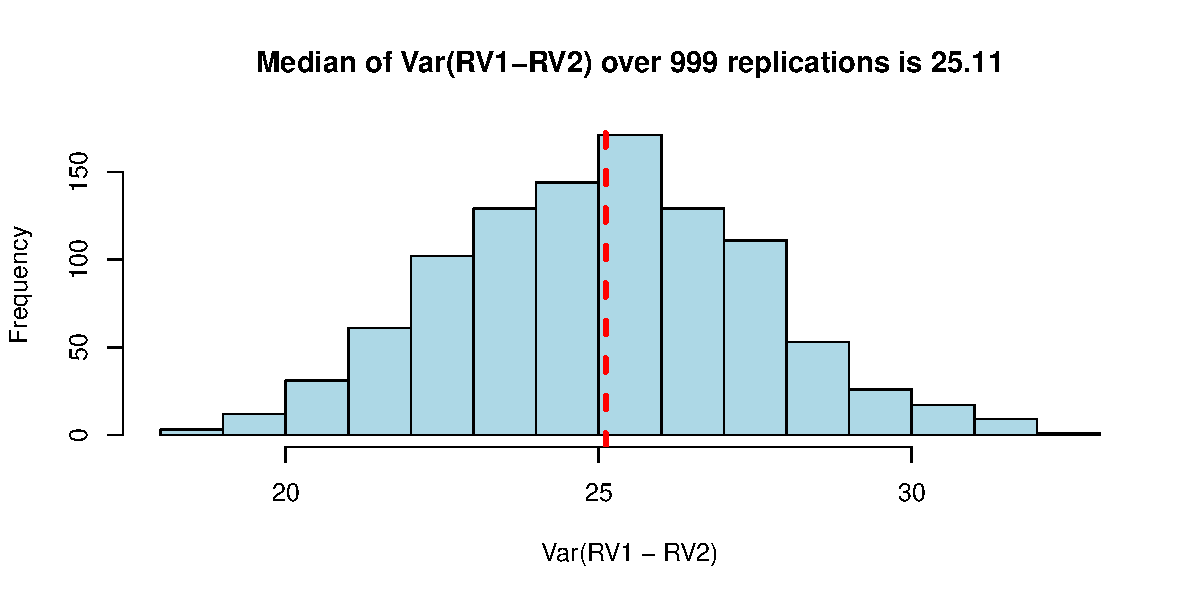
\includegraphics[width=\maxwidth]{figure/unnamed-chunk-15-1} 

}


\end{knitrout}
\end{frame}

\section{Sampling Distributions, CLT, Confidence Intervals and p-values}


\begin{frame}{Parameters,  Samples,  and  Statistics}
	\begin{itemize}
		\item \textbf{Paramter}: An  unknown  numerical  constant  pertaining  to  a  population/universe,  or  in  a  statistical  model. 
		\begin{itemize}
			\item $\mu$: population mean $\qquad\qquad$ $\pi$: population proportion
		\end{itemize}
		
		\item \textbf{Statistic}: A  numerical  quantity  calculated  from  a  sample. The  empirical counterpart of the parameter,  used  to  \textit{estimate}  it.
		
		\begin{itemize}
			\item $\bar{y}$: sample mean $\qquad\qquad$ $p$: sample proportion
		\end{itemize}
	\end{itemize}
	
	\pause
	\Wider[4em]{
		\centering
		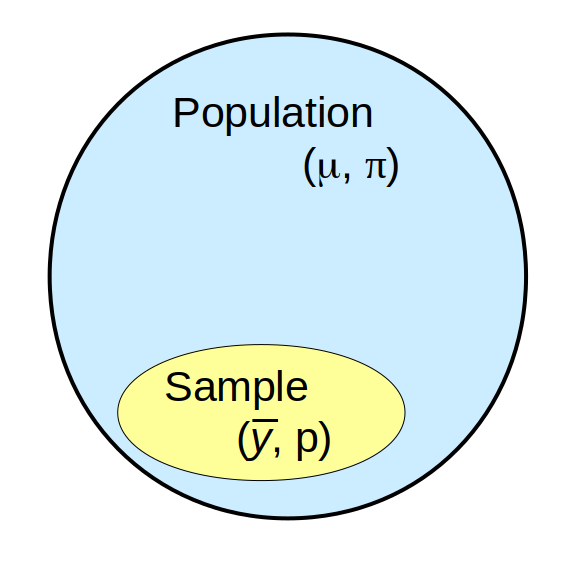
\includegraphics[scale=0.35]{MeansFig1.png}
	}
	
	
\end{frame}


\frame{\frametitle{Samples must be random} 
	
	\begin{itemize}
		\item 	The validity of inference will depend on the
		way that the sample was collected. If a sample was collected badly, no amount of
		statistical sophistication can rescue the study. \\ \ \\ 
		
		\item Samples should be \textbf{random}. That is, there should be no systematic set of
		characteristics that is related to the scientific question of interest that causes some
		people to be more likely to be sampled than others. The simplest type of randomization
		selects members from the population with equal probability (a uniform distribution). \\ \
		\\ 
		
		\pause
		
		\item 	\textbf{Do not cheat by}  
		\begin{itemize}
			\item 	Taking 5 people from the \emph{same} household to estimate
			
			\begin{itemize}
				\item proportion of Québécois who don't have a family doctor
				\item who saw a medical doctor last year
				\item average rent
			\end{itemize}  
			
			
			
			
			\item Sampling the depth of the ocean \emph{only around Montreal} to estimate \begin{itemize}
				\item proportion of  Earth's  surface  covered  by  water
			\end{itemize} 
			
		\end{itemize}
	\end{itemize}
}






\frame{\frametitle{Sampling Distributions} 
	
	\begin{definition}[Sampling Distribution]
		\begin{itemize}
			\setlength\itemsep{1.5em}
			\item The sampling distribution of a statistic is the distribution of values taken by the statistic in \textbf{all possible samples of the same size} from the same population.
			\item The standard deviation of a sampling distribution is called a \textbf{standard error}
		\end{itemize} 
	\end{definition}
	
	
	
}


\begin{frame}[fragile]{Sampling Distributions}
	
\begin{knitrout}\tiny
\definecolor{shadecolor}{rgb}{0.969, 0.969, 0.969}\color{fgcolor}\begin{figure}

{\centering 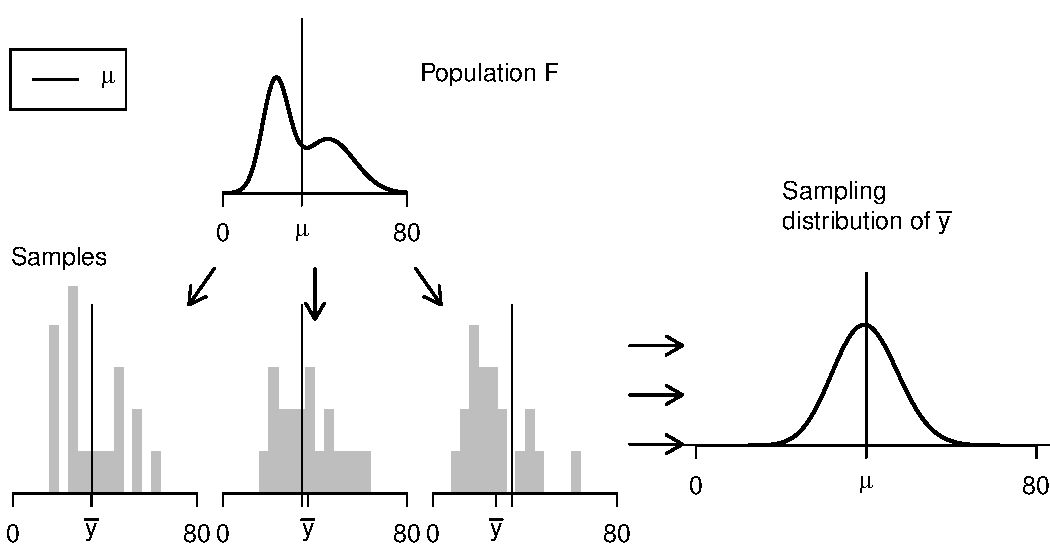
\includegraphics[width=\maxwidth]{figure/unnamed-chunk-16-1} 

}

\caption[Ideal world]{Ideal world. Sampling distributions are obtained by drawing repeated samples from the population, computing the statistic of interest for each, and collecting (an infinite number of) those statistics as the sampling distribution}\label{fig:unnamed-chunk-16}
\end{figure}

\end{knitrout}
	
\end{frame}


\frame{\frametitle{Why are sampling distributions important?} 
	
	\begin{itemize}
		\setlength\itemsep{2em} 
		\item They  tell  us  how  far  from  the  target  (true  value  of  the  parameter)  our  statistical  \emph{shot}  at  it  (i.e.  the  statistic  calculated  form  a  sample)  is  likely  to  be,  or, to  have  been.  \pause 
		
		\item Thus,  they  are  used  in  confidence  intervals  for  parameters. Specific  sampling  distributions  (based  on  a null value  for  the  parameter)  are also  used  in  statistical  tests  of  hypotheses.
		
	\end{itemize}	
	
	
}


\begin{frame}[fragile]{Sampling distribution: mean depth of the ocean}
	

	
\begin{knitrout}\tiny
\definecolor{shadecolor}{rgb}{0.969, 0.969, 0.969}\color{fgcolor}

{\centering 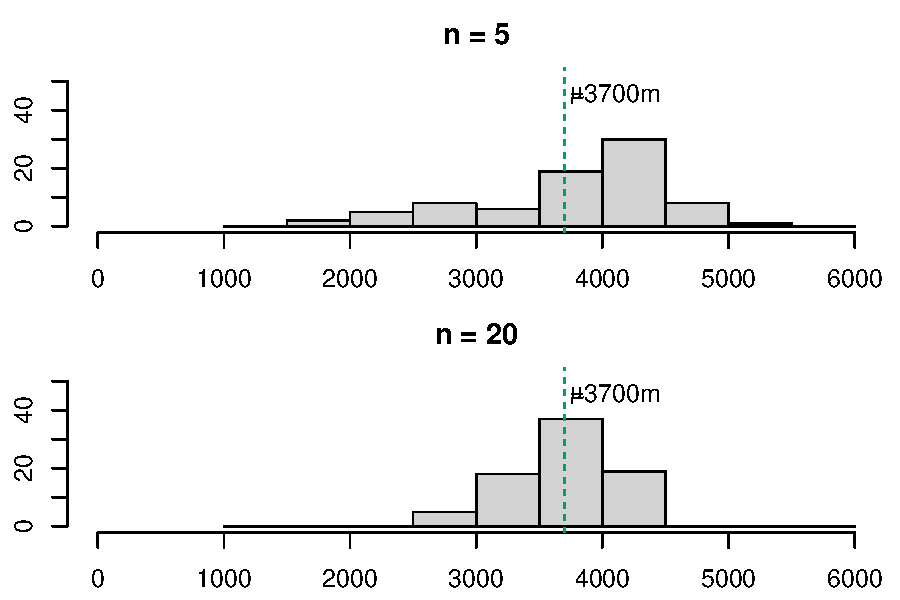
\includegraphics[width=\maxwidth]{figure/unnamed-chunk-18-1} 

}


\end{knitrout}
	
\end{frame}



\begin{frame}[fragile]{Sampling distribution: proportion covered by water}
	

	
	
\begin{knitrout}\tiny
\definecolor{shadecolor}{rgb}{0.969, 0.969, 0.969}\color{fgcolor}

{\centering 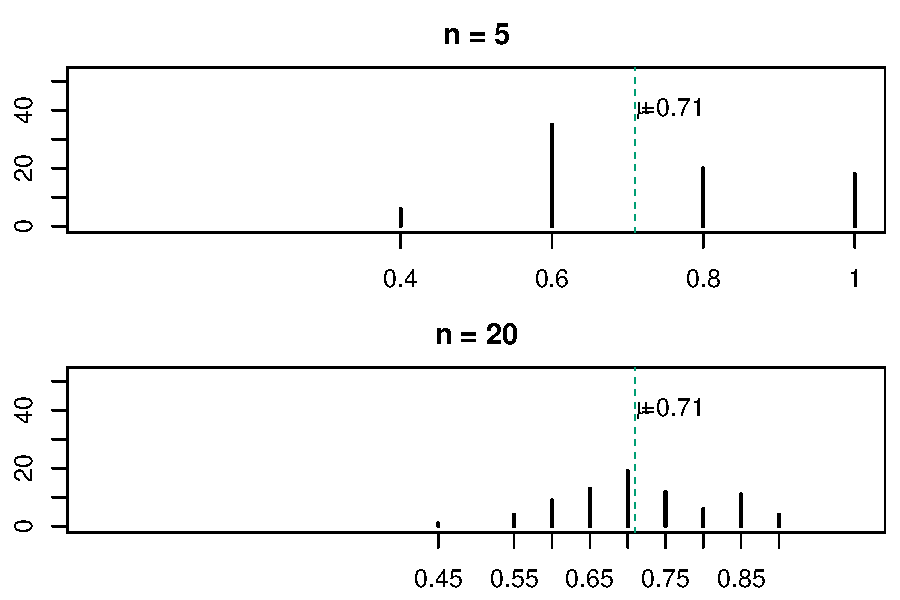
\includegraphics[width=\maxwidth]{figure/unnamed-chunk-20-1} 

}


\end{knitrout}
	
\end{frame}




\begin{frame}[fragile]{Normal Distribution: For probabilities we use $pnorm$}
	
	
\begin{knitrout}\tiny
\definecolor{shadecolor}{rgb}{0.969, 0.969, 0.969}\color{fgcolor}\begin{kframe}
\begin{alltt}
\hlstd{stats}\hlopt{::}\hlkwd{pnorm}\hlstd{(}\hlkwc{q} \hlstd{=} \hlnum{130}\hlstd{,} \hlkwc{mean} \hlstd{=} \hlnum{100}\hlstd{,} \hlkwc{sd} \hlstd{=} \hlnum{13}\hlstd{)}
\end{alltt}
\begin{verbatim}
## [1] 0.9894919
\end{verbatim}
\end{kframe}
\end{knitrout}
	
	
\begin{knitrout}\tiny
\definecolor{shadecolor}{rgb}{0.969, 0.969, 0.969}\color{fgcolor}\begin{kframe}
\begin{alltt}
\hlstd{mosaic}\hlopt{::}\hlkwd{xpnorm}\hlstd{(}\hlkwc{q} \hlstd{=} \hlnum{130}\hlstd{,} \hlkwc{mean} \hlstd{=} \hlnum{100}\hlstd{,} \hlkwc{sd} \hlstd{=} \hlnum{13}\hlstd{)}
\end{alltt}
\end{kframe}

{\centering 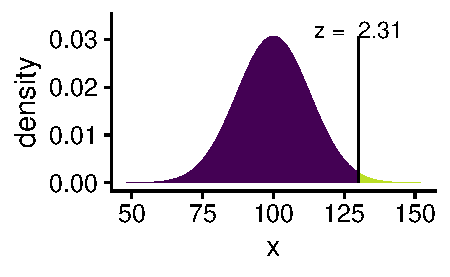
\includegraphics[width=0.6\linewidth]{figure/probs3-1} 

}


\begin{kframe}\begin{verbatim}
## [1] 0.9894919
\end{verbatim}
\end{kframe}
\end{knitrout}
	
	
	\begin{itemize}
		\item \texttt{pnorm} returns the integral from $-\infty$ to $q$ for a $\mathcal{N}(\mu, \sigma)$
		\item \texttt{pnorm} goes from \textit{quantiles} (think $Z$ scores) to probabilities
	\end{itemize}
	
\end{frame}



\begin{frame}[fragile]{Normal Distribution: For quantiles we use $qnorm$}
	
	
	
\begin{knitrout}\tiny
\definecolor{shadecolor}{rgb}{0.969, 0.969, 0.969}\color{fgcolor}\begin{kframe}
\begin{alltt}
\hlstd{stats}\hlopt{::}\hlkwd{qnorm}\hlstd{(}\hlkwc{p} \hlstd{=} \hlnum{0.0104}\hlstd{,} \hlkwc{mean} \hlstd{=} \hlnum{100}\hlstd{,} \hlkwc{sd} \hlstd{=} \hlnum{13}\hlstd{)}
\end{alltt}
\begin{verbatim}
## [1] 69.94926
\end{verbatim}
\end{kframe}
\end{knitrout}
	
	
	
\begin{knitrout}\tiny
\definecolor{shadecolor}{rgb}{0.969, 0.969, 0.969}\color{fgcolor}\begin{kframe}
\begin{alltt}
\hlstd{mosaic}\hlopt{::}\hlkwd{xqnorm}\hlstd{(}\hlkwc{p} \hlstd{=} \hlnum{0.0104}\hlstd{,} \hlkwc{mean} \hlstd{=} \hlnum{100}\hlstd{,} \hlkwc{sd} \hlstd{=} \hlnum{13}\hlstd{)}
\end{alltt}
\end{kframe}

{\centering 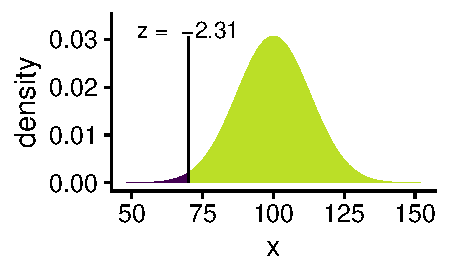
\includegraphics[width=0.6\linewidth]{figure/probs5-1} 

}


\begin{kframe}\begin{verbatim}
## [1] 69.94926
\end{verbatim}
\end{kframe}
\end{knitrout}
	
	
	
	\small{
		\begin{itemize}
			\item \texttt{qnorm} answers the question: What is the Z-score of the $p$th percentile of the normal distribution?
			
			\item \texttt{qnorm} goes from \textit{probabilities} to quantiles 
		\end{itemize}
	}
\end{frame}

\begin{frame}[fragile]{Empirical Rule or 68-95-99.7\% Rule}
	
	\framedgraphic{6899rule.png}
	
\end{frame}



\begin{frame}[fragile]{Quadruple the work, half the benefit}
	
	\framedgraphiccaption{ROOToceanAll.png}{When the sample size increases from 4 to 16, the spread of the sampling distribution for the mean is reduced by a half, i.e., the range is cut in half. This is known as the curse of the $\sqrt{n}$}
\end{frame}


\frame{\frametitle{The Central Limit Theorem (CLT)} 
	
	\begin{itemize}
		\item The sampling distribution of $\bar{y}$ is, for a large enough $n$, close to Gaussian in shape no matter what the shape of the distribution of individual $Y$ values. 
		\item This phenomenon is referred to as the CENTRAL LIMIT THEOREM 
		\item The CLT applied also to a \underline{sample proportion}, \underline{slope}, \underline{correlation}, or any other statistic created by \underline{aggregation of individual observations}
	\end{itemize}
	
	\begin{theorem}[Central Limit Theorem]
		\begin{center}
			if $Y \sim ???(\mu_Y, \sigma_Y)$, then \\ \ \\
			$\bar{y} \sim \mathcal{N}(\mu_Y, \sigma_Y / \sqrt{n})$
		\end{center}
	\end{theorem}
	
	\vspace{1.25cm}
	%pause
}



\begin{frame}[fragile,plain]

	
	
\begin{knitrout}\tiny
\definecolor{shadecolor}{rgb}{0.969, 0.969, 0.969}\color{fgcolor}\begin{figure}

{\centering 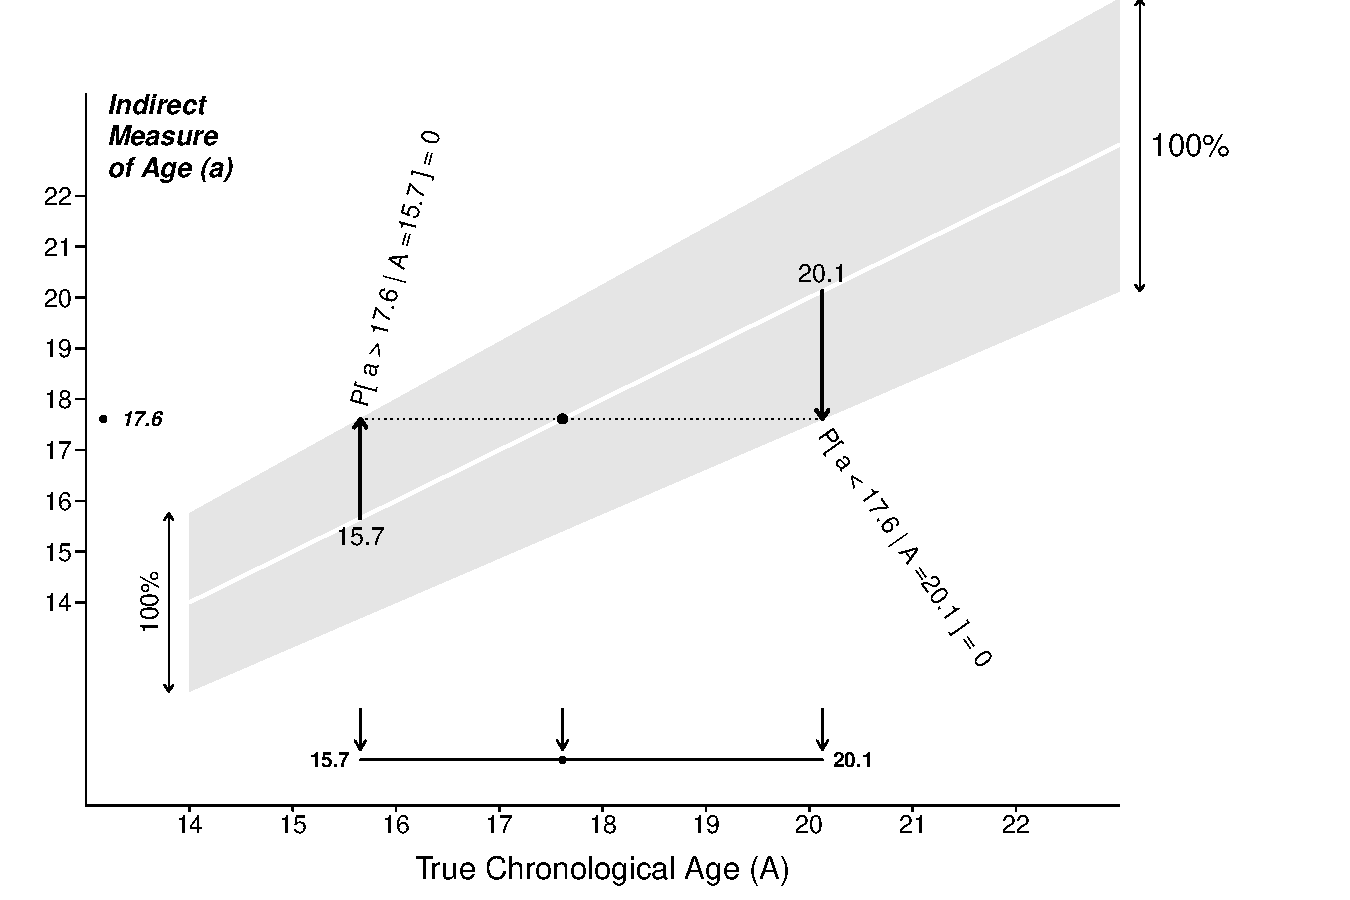
\includegraphics[width=\maxwidth]{figure/unnamed-chunk-22-1} 

}

\caption[100\% Confidence Intervals for a person's chronological age when error distributions (that in this example are wider at the  older ages) are 100\% confined within the shaded ranges]{100\% Confidence Intervals for a person's chronological age when error distributions (that in this example are wider at the  older ages) are 100\% confined within the shaded ranges. }\label{fig:unnamed-chunk-22}
\end{figure}

\end{knitrout}
	
	
\end{frame}


\begin{frame}{Confidence Interval}
	
	\begin{definition}[Confidence Interval]
		A level $C$ confidence interval for a parameter has two parts:
		\begin{enumerate}
			\item An interval calculated from the data, \underline{usually} of the form $$\textrm{estimate} \pm \textrm{margin of error}$$ where the estimate is a sample statistic and the margin of error represents the accuracy of our guess for the parameter.
			\item A confidence level $C$, which gives the probability that the interval will capture the true parameter value in \textit{different possible samples}. That is, the confidence level is the success rate for the method
		\end{enumerate}
	\end{definition}
	
	%\framedgraphic{6899rule.png}
	
\end{frame}

\frame{\frametitle{Confidence Interval: A simulation study}
	
	\vspace*{-0.1in}
	
	\begin{figure}
		\begin{center}
			\epsfig{figure=CIplots.eps,width=3.2in,height=2.7in}
			\caption{\small{True parameter value is 2 (red line). Each horizontal black line represents a 95\% CI from a sample and contains the true parameter value. The blue CIs do not contain the true parameter value. 95\% of all samples give an interval that contains the population parameter.}}
		\end{center}
	\end{figure}
}


\begin{frame}{Interpreting a frequentist confidence interval}
	\begin{itemize}
		\setlength\itemsep{1em}
		\item The confidence level is the success rate of the method that produces the interval. 
		\item We don't know whether the 95\% confidence interval from a \underline{particular
			sample} is one of the 95\% that capture $\theta$ (the unknown population parameter), or one of the unlucky 5\% that miss. 
		\item To say that we are \underline{95\% confident} that the unknown value of $\theta$
		lies between $U$ and $L$ is shorthand for ``We got these numbers using a
		method that gives correct results 95\% of the time.''
	\end{itemize}
\end{frame}

\begin{frame}[fragile]{68\% Confidence interval using \texttt{qnorm}}
	

	
	
	\vspace*{-0.09in}
	
	\Wider[2em]{
\begin{knitrout}\tiny
\definecolor{shadecolor}{rgb}{0.969, 0.969, 0.969}\color{fgcolor}\begin{figure}

{\centering 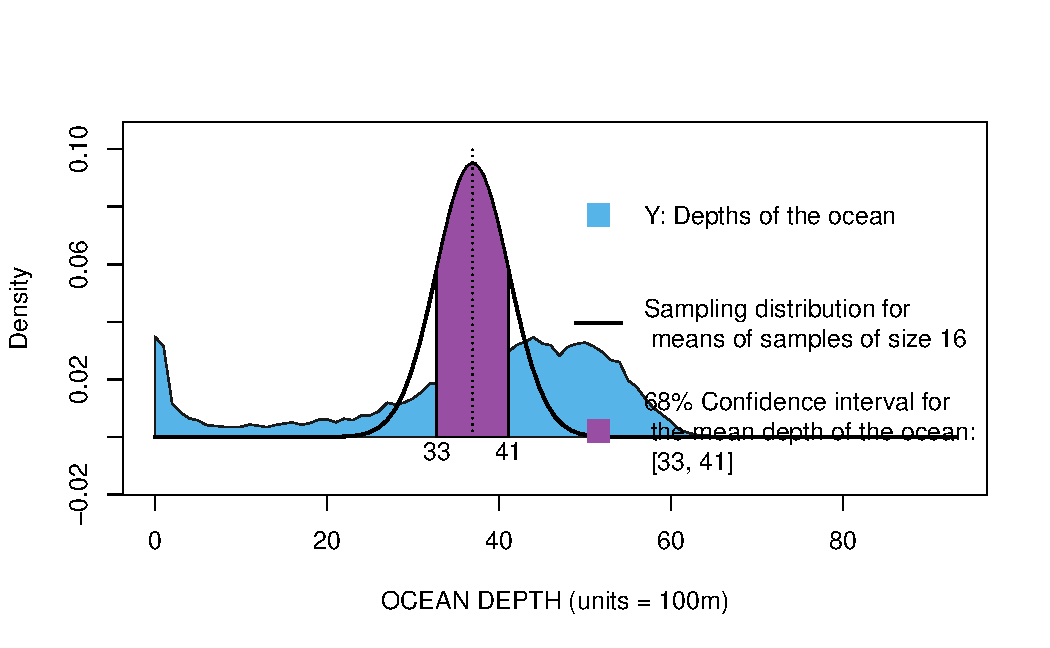
\includegraphics[width=\maxwidth]{figure/unnamed-chunk-24-1} 

}

\caption{68\% Confidence interval calculated using  \mbox{\texttt{qnorm(p = c(0.16,0.84), mean = 37, sd = 4.2)}}}\label{fig:unnamed-chunk-24}
\end{figure}

\end{knitrout}
		
	}
\end{frame}



\begin{frame}[fragile]{95\% Confidence interval using \texttt{qnorm}}
	
	\vspace*{-0.09in}
	
	
	\Wider[2em]{
\begin{knitrout}\tiny
\definecolor{shadecolor}{rgb}{0.969, 0.969, 0.969}\color{fgcolor}\begin{figure}

{\centering 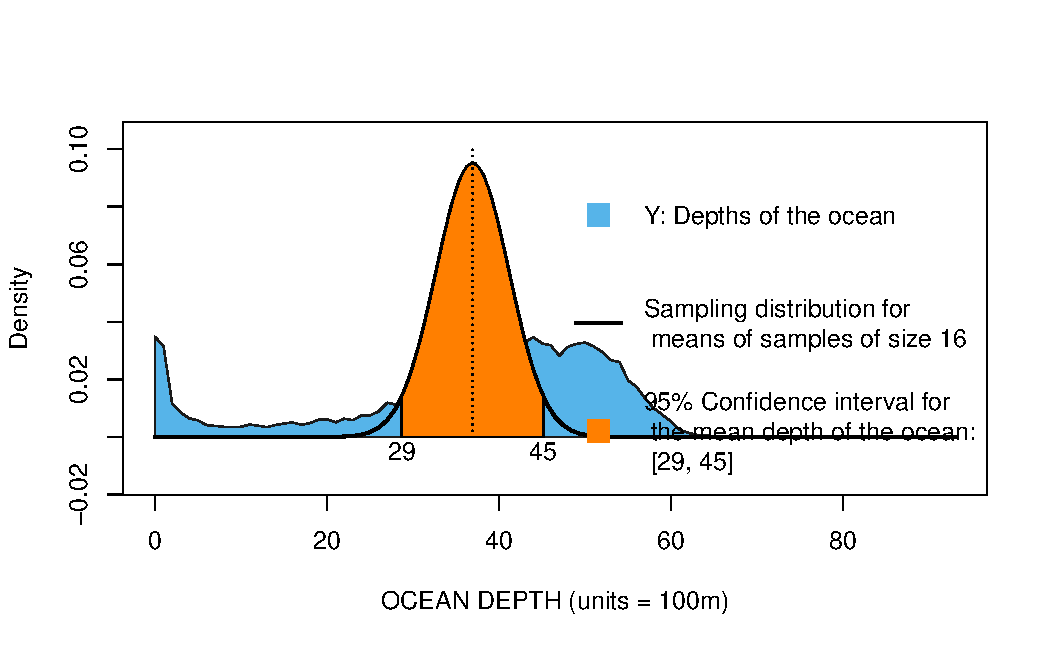
\includegraphics[width=\maxwidth]{figure/unnamed-chunk-25-1} 

}

\caption{95\% Confidence interval calculated using  \mbox{\texttt{qnorm(p = c(0.025,0.975), mean = 37, sd = 4.2)}}}\label{fig:unnamed-chunk-25}
\end{figure}

\end{knitrout}
		
	}
	
\end{frame}

\frame{\frametitle{Example: Inference for a single population mean} So what
	does the CI allow us to learn about $\mu$??
	\begin{itemize}
		\setlength\itemsep{2em}
		\item It tells us that if we repeated this procedure again and again
		(collecting a sample mean, and constructing a 95\% CI), 95\% of the
		time, the CI would \textit{cover} $\mu$. 
		\item That is, with 95\% probability, the \textit{procedure}
		will include the true value of $\mu$. Note that we are making \underline{a probability statement about the CI}, not about the parameter. 
		\item Unfortunately, \textcolor{blue}{we do not know whether the true value of $\mu$ is
			contained in the CI in the particular experiment that we have
			performed.}
	\end{itemize}
}



\section{Bootstrap}

\begin{frame}{Motivation for the Bootstrap}
	\begin{itemize}
		\setlength\itemsep{2em}
		\item The $\pm$ and \texttt{qnorm}/\texttt{qt} methods to calculate a CI both require the CLT
	\end{itemize}
	
	
	
	\vspace*{0.2in}
	
	\Large \textcolor{myblue}{Q: What happens if the CLT hasn't `kicked in`? Or you don't believe the CLT?} \\ \ \\
	\pause 
	\Large \textcolor{myblue}{Q: What happens if there is no formula available to calculate a CI?} \\ \ \\
	\pause 
	\Large \textcolor{red}{A: Bootstrap} \\ \ \\
\end{frame}



\begin{frame}[fragile]{Ideal world: known sampling distribution}
	
\begin{knitrout}\tiny
\definecolor{shadecolor}{rgb}{0.969, 0.969, 0.969}\color{fgcolor}\begin{figure}

{\centering 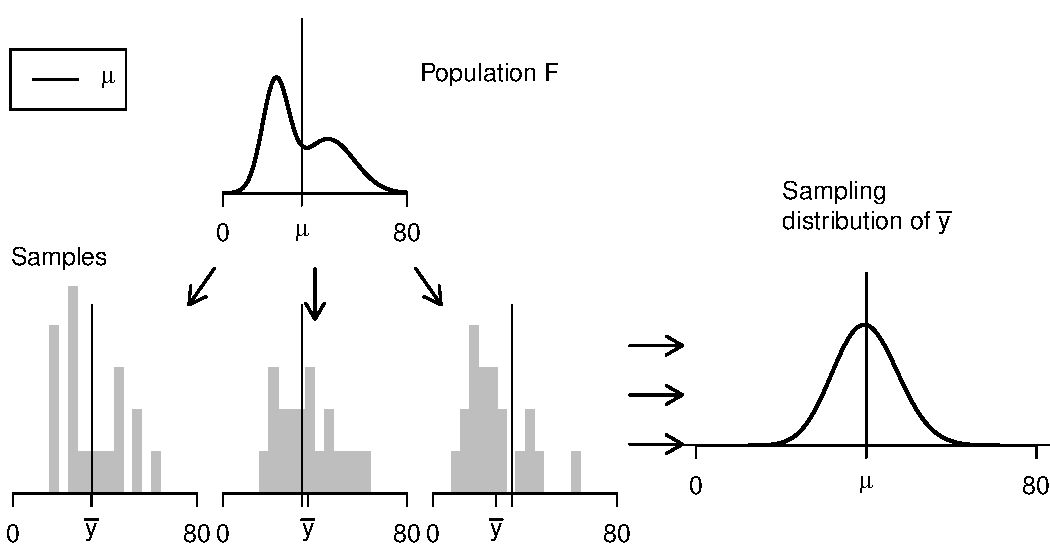
\includegraphics[width=\maxwidth]{figure/unnamed-chunk-26-1} 

}

\caption{\scriptsize{Ideal world. Sampling distributions are obtained by drawing repeated samples from the population, computing the statistic of interest for each, and collecting (an infinite number of) those statistics as the sampling distribution}}\label{fig:unnamed-chunk-26}
\end{figure}

\end{knitrout}
	
\end{frame}



\begin{frame}[fragile]{Reality: use the bootstrap distribution instead}
	
	

	
	\framedgraphiccaption{boot_diag.pdf}{\scriptsize{Bootstrap world. The bootstrap distribution is obtained by drawing repeated samples from an estimate of the population, computing the statistic of interest for each, and collecting those statistics. The distribution is centered at the observed statistic ($\bar{y}$), not the parameter ($\mu$).}}
	
\end{frame}


\begin{frame}[fragile]{Main idea: simulate your own sampling distribution}
	

	
\begin{knitrout}\tiny
\definecolor{shadecolor}{rgb}{0.969, 0.969, 0.969}\color{fgcolor}\begin{kframe}
\begin{alltt}
\hlstd{R} \hlkwb{<-} \hlkwd{replicate}\hlstd{(B, \{}
\hlstd{dplyr}\hlopt{::}\hlkwd{sample_n}\hlstd{(depths.n.20,} \hlkwc{size} \hlstd{= N,} \hlkwc{replace} \hlstd{=} \hlnum{TRUE}\hlstd{)} \hlopt
\hlstd{dplyr}\hlopt{::}\hlkwd{summarize}\hlstd{(}\hlkwc{r} \hlstd{=} \hlkwd{mean}\hlstd{(alt))} \hlopt
\hlstd{dplyr}\hlopt{::}\hlkwd{pull}\hlstd{(r)}
\hlstd{\})}
\hlstd{CI_95} \hlkwb{<-} \hlkwd{quantile}\hlstd{(R,} \hlkwc{probs} \hlstd{=} \hlkwd{c}\hlstd{(}\hlnum{0.025}\hlstd{,} \hlnum{0.975}\hlstd{))}
\end{alltt}
\end{kframe}

{\centering 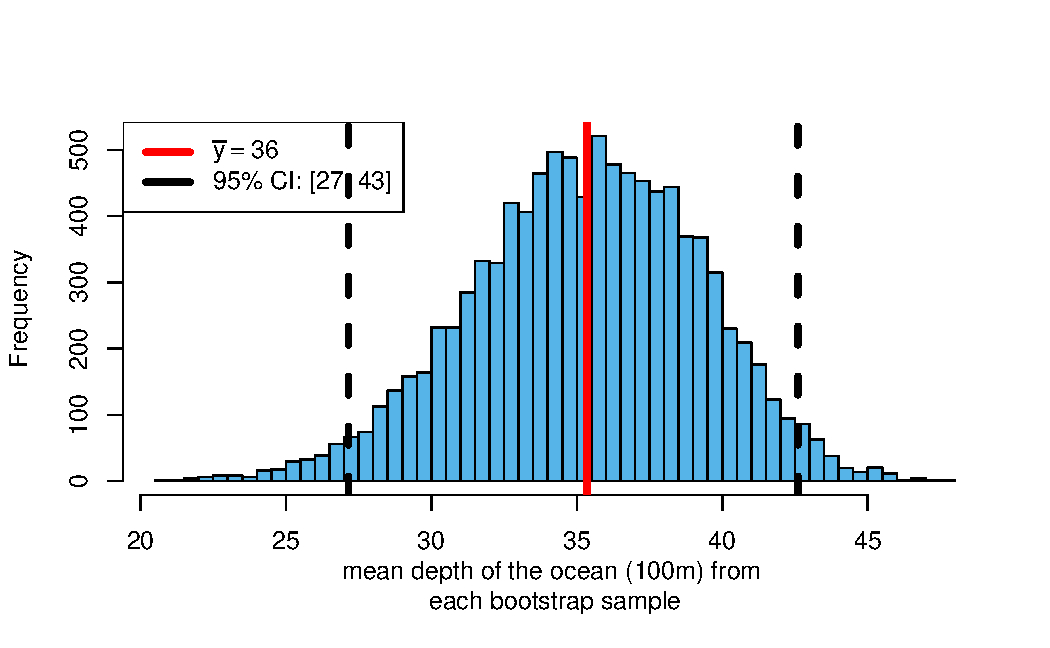
\includegraphics[width=\maxwidth]{figure/unnamed-chunk-29-1} 

}


\end{knitrout}
	
\end{frame}

\begin{frame}{Bootstrap can be used for other statistics (e.g. $R^2$)}
	\centering
	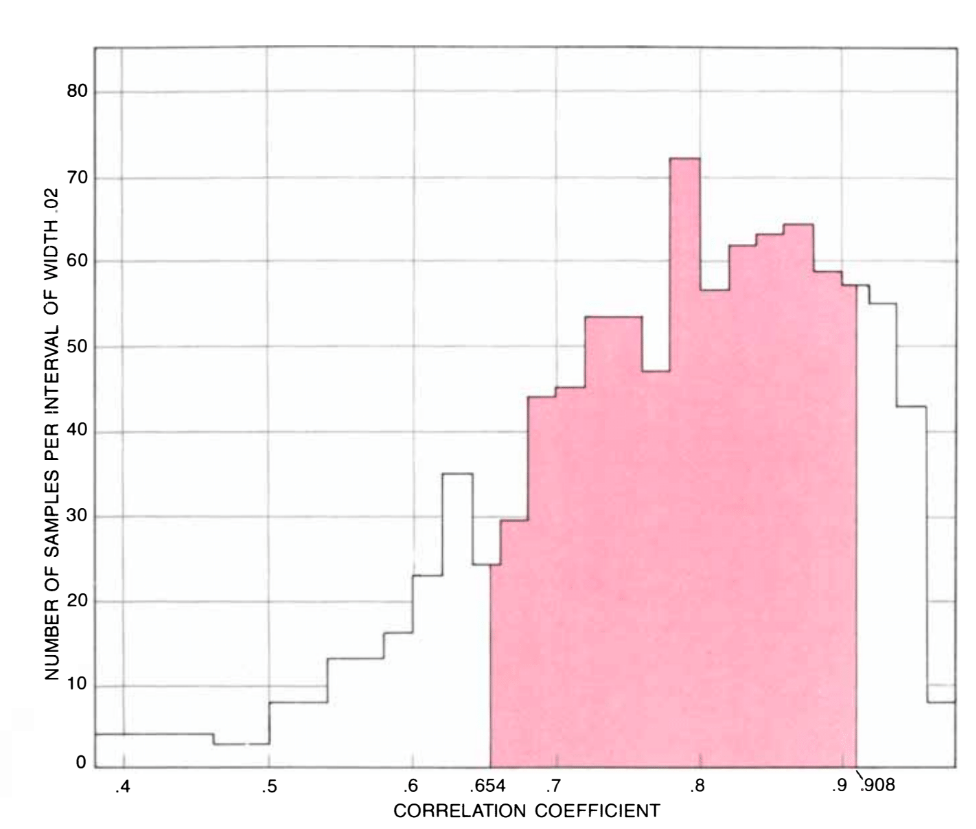
\includegraphics[scale=0.29]{bootcorr.png}
	
	\vspace{0.1in}
	
	\tiny \href{https://www.dropbox.com/s/cxiq70zxxtyxlb5/EfronDiaconisBootstrap.pdf?dl=0}{source: Bootstrap article in Scientific American}
\end{frame}


\section{One sample mean}


\begin{frame}{$\sigma$ known vs. unknown}
	\begin{center}
		\begin{tabular}{|l|c|c|} \hline
			$\sigma$& known & unknown \\ \hline Data & $\{y_1,y_2,...,y_n\}$ &
			$\{y_1,y_2,...,y_n\}$\\
			& & \\
			Pop'n param & $\mu$ & $\mu$\\
			& & \\
			Estimator & $\overline{y} = \frac{1}{n}\sum_{i=1}^n y_i$ & $\overline{y} = \frac{1}{n}\sum_{i=1}^n y_i$ \\
			& & \\
			SD & $\sigma$ & $s = \sqrt{\frac{\sum_{i=1}^n(y_i-\overline{y})^2}{n-1}}$ \\
			& & \\
			SEM & $\sigma/\sqrt{n}$ & $s / \sqrt{n}$ \\
			& & \\
			$(1-\alpha)100$\% CI & $\overline{y} \pm z^\star_{1-\alpha/2}$(SEM) & $\overline{y} \pm t^\star_{1-\alpha/2, (n-1)}$(SEM) \\
			& & \\
			test statistic & $\frac{\overline{y}-\mu_0}{\textrm{SEM}}\sim \mathcal{N}(0,1)$ &
			$\frac{\overline{y}-\mu_0}{\textrm{SEM}}\sim t_{(n-1)}$ \\
			\hline
		\end{tabular}
	\end{center}
\end{frame}


\begin{frame}{Assumptions}
	\Wider[3em]{
		\begin{center}
			\begin{tabular}{|l|c|c|c|} \hline
				& $z$ & $t$ & Bootstrap \\ 
				\hline 
				SRS & \cmark &\cmark &	\cmark\\
				& & & \\
				Normal population & \cmark$^\star$ & \cmark$^\star$ &  \xmark\\
				& & &\\
				needs CLT &  \cmark$^\star$ & \cmark$^\star$ &  \xmark\\
				& & &\\
				$\sigma$ known  & \cmark & \xmark & \xmark\\
				& & &\\
				Sampling dist. center at & $\mu$ & $\mu$ & $\bar{y}$\\
				& & &\\
				SD & $\sigma$ & $s$ & $s$ \\
				& & &\\
				SEM & $\sigma/\sqrt{n}$ & $s / \sqrt{n}$ & SD(bootstrap statistics) \\
				\hline
			\end{tabular}
			
			\footnotetext[1]{*If population is Normal then CLT is not needed. If population is not Normal then CLT is needed.}
		\end{center}
	}
\end{frame}


\begin{frame}[fragile]{Application: How fast is your reaction time?}
\begin{knitrout}\tiny
\definecolor{shadecolor}{rgb}{0.969, 0.969, 0.969}\color{fgcolor}\begin{kframe}
\begin{alltt}
\hlstd{reaction.times} \hlkwb{<-} \hlkwd{c}\hlstd{(}\hlnum{325}\hlstd{,}\hlnum{327}\hlstd{,}\hlnum{357}\hlstd{,}\hlnum{299}\hlstd{,}\hlnum{378}\hlstd{)}\hlopt{/}\hlnum{1000}
\hlkwd{summary}\hlstd{(reaction.times)}
\end{alltt}
\begin{verbatim}
##    Min. 1st Qu.  Median    Mean 3rd Qu.    Max. 
##  0.2990  0.3250  0.3270  0.3372  0.3570  0.3780
\end{verbatim}
\begin{alltt}
\hlkwd{round}\hlstd{(}\hlkwd{sd}\hlstd{(reaction.times),}\hlnum{3}\hlstd{)}
\end{alltt}
\begin{verbatim}
## [1] 0.031
\end{verbatim}
\begin{alltt}
\hlkwd{length}\hlstd{(reaction.times)}
\end{alltt}
\begin{verbatim}
## [1] 5
\end{verbatim}
\end{kframe}
\end{knitrout}
	
\end{frame}


\begin{frame}[fragile]{5 ways of calculating a confidence interval}
	
	We are interested in calculating a 95\% confidence interval for the mean reaction time based on the sample of 5 reaction times. \\ \ \\
	\pause
	Five ways of doing this:
	\begin{enumerate}
		\setlength\itemsep{1em}
		\item By hand (using the $\pm$ formula and \texttt{R} as a calculator)
		\item Using the quantile function for the $t$ distribution \texttt{stats::qt}
		\item Fitting an intercept-only regression model ($y = \beta_0 + \varepsilon$)
		\item Using a canned function (\texttt{mosaic::t.test}, \texttt{stats::t.test})
		\item Bootstrap
	\end{enumerate}
	
\end{frame}

\begin{frame}[fragile]{1. By hand using the $\pm$ formula}
\begin{knitrout}\tiny
\definecolor{shadecolor}{rgb}{0.969, 0.969, 0.969}\color{fgcolor}\begin{kframe}
\begin{alltt}
\hlstd{n} \hlkwb{<-} \hlkwd{length}\hlstd{(reaction.times)}
\hlstd{SEM} \hlkwb{<-} \hlkwd{sd}\hlstd{(reaction.times)}\hlopt{/}\hlkwd{sqrt}\hlstd{(n)}
\end{alltt}
\begin{verbatim}
## [1] 0.01372734
\end{verbatim}
\begin{alltt}
\hlstd{ybar} \hlkwb{<-} \hlkwd{mean}\hlstd{(reaction.times)}
\end{alltt}
\begin{verbatim}
## [1] 0.3372
\end{verbatim}
\begin{alltt}
\hlstd{multiple.for.95pct} \hlkwb{<-} \hlstd{stats}\hlopt{::}\hlkwd{qt}\hlstd{(}\hlkwc{p} \hlstd{=} \hlkwd{c}\hlstd{(}\hlnum{0.025}\hlstd{,} \hlnum{0.975}\hlstd{),} \hlkwc{df} \hlstd{= n}\hlopt{-}\hlnum{1}\hlstd{)}
\end{alltt}
\begin{verbatim}
## [1] -2.776445  2.776445
\end{verbatim}
\begin{alltt}
\hlstd{by_hand_CI} \hlkwb{<-} \hlstd{ybar} \hlopt{+} \hlstd{multiple.for.95pct} \hlopt{*} \hlstd{SEM}
\end{alltt}
\begin{verbatim}
## [1] 0.29909 0.37531
\end{verbatim}
\end{kframe}
\end{knitrout}
\end{frame}

\begin{frame}[fragile]{2. Using \texttt{stats::qt}}
	\textit{Note: \texttt{R} only provides the standard $t$ distribution. In order to get a scaled version we must define our own function.}
	
	\vspace*{0.2in}
	
\begin{knitrout}\tiny
\definecolor{shadecolor}{rgb}{0.969, 0.969, 0.969}\color{fgcolor}\begin{kframe}
\begin{alltt}
\hlstd{n} \hlkwb{<-} \hlkwd{length}\hlstd{(reaction.times)}
\hlstd{SEM} \hlkwb{<-} \hlkwd{sd}\hlstd{(reaction.times)}\hlopt{/}\hlkwd{sqrt}\hlstd{(n)}
\hlstd{ybar} \hlkwb{<-} \hlkwd{mean}\hlstd{(reaction.times)}

\hlcom{# scaled version of the standard t distribution}
\hlstd{qt_ls} \hlkwb{<-} \hlkwa{function}\hlstd{(}\hlkwc{p}\hlstd{,} \hlkwc{df}\hlstd{,} \hlkwc{mean}\hlstd{,} \hlkwc{sd}\hlstd{)} \hlkwd{qt}\hlstd{(}\hlkwc{p} \hlstd{= p,} \hlkwc{df} \hlstd{= df)} \hlopt{*} \hlstd{sd} \hlopt{+} \hlstd{mean}

\hlkwd{qt_ls}\hlstd{(}\hlkwc{p} \hlstd{=} \hlkwd{c}\hlstd{(}\hlnum{0.025}\hlstd{,} \hlnum{0.975}\hlstd{),} \hlkwc{df} \hlstd{= n} \hlopt{-} \hlnum{1}\hlstd{,} \hlkwc{mean} \hlstd{= ybar,} \hlkwc{sd} \hlstd{= SEM)}
\end{alltt}
\begin{verbatim}
## [1] 0.2990868 0.3753132
\end{verbatim}
\end{kframe}
\end{knitrout}
\end{frame}


\begin{frame}[fragile]{3. Fitting an intercept-only regression model}
\begin{knitrout}\tiny
\definecolor{shadecolor}{rgb}{0.969, 0.969, 0.969}\color{fgcolor}\begin{kframe}
\begin{alltt}
\hlstd{fit} \hlkwb{<-} \hlstd{stats}\hlopt{::}\hlkwd{lm}\hlstd{(reaction.times} \hlopt{~} \hlnum{1}\hlstd{)}
\hlkwd{summary}\hlstd{(fit)}
\end{alltt}
\begin{verbatim}
## Coefficients:
##             Estimate Std. Error t value Pr(>|t|)    
## (Intercept)  0.33720    0.01373   24.56 1.63e-05 ***
## ---
## Signif. codes:  0 '***' 0.001 '**' 0.01 '*' 0.05 '.' 0.1 ' ' 1
## 
## Residual standard error: 0.0307 on 4 degrees of freedom
\end{verbatim}
\begin{alltt}
\hlstd{stats}\hlopt{::}\hlkwd{confint}\hlstd{(fit)}
\end{alltt}
\begin{verbatim}
##                 2.5 %    97.5 %
## (Intercept) 0.2990868 0.3753132
\end{verbatim}
\end{kframe}
\end{knitrout}
\end{frame}


\begin{frame}[fragile]{3. Fitting an intercept-only regression model}
	In the regression output:
	\begin{itemize}
		\setlength\itemsep{1em}
		\item \texttt{Estimate}: the mean reaction time (an estimate of the intercept $\beta_0$)
		\item \texttt{t value}: the test statistic 
		\item \texttt{Std. Error}: the standard error of the mean (SEM)
		\item \texttt{Pr(>|t|)}: is the $p$-value
	\end{itemize} 
	
	
\end{frame}


\begin{frame}[fragile]{3. Fitting an intercept-only regression model}
	

	
	\small
	These are based on the (useless) null hypothesis $H_0: \mu_0 = 0$ \\ \ \\
	
	\begin{itemize}
		\item \texttt{t value} = $\frac{\bar{y} - \mu_0}{s / \sqrt{n}}$ = $\frac{0.33720 - 0}{0.01373}$ = 24.56
		\item \texttt{Pr(>|t|)} \\ \ \\
		= $P(\textrm{t value} > t_{(n-1)}) + P(-\textrm{t value} < t_{(n-1)})$ \\ \ \\
		= \small{\texttt{pt(q = 24.56, df = n-1, lower.tail = FALSE)} +  \texttt{pt(q = -24.56, df = n-1)}} \\ \ \\
		= \ensuremath{8.155\times 10^{-6}} + \ensuremath{8.155\times 10^{-6}} = \ensuremath{1.631\times 10^{-5}}
	\end{itemize}
	
	
\end{frame}



\begin{frame}[fragile]{4. Canned function}
	
\begin{knitrout}\tiny
\definecolor{shadecolor}{rgb}{0.969, 0.969, 0.969}\color{fgcolor}\begin{kframe}
\begin{alltt}
\hlstd{stats}\hlopt{::}\hlkwd{t.test}\hlstd{(reaction.times)}
\end{alltt}
\begin{verbatim}
## One Sample t-test with reaction.times 
## t = 24.6, df = 4, p-value = 1.63e-05
## alternative hypothesis: true mean is not equal to 0 
## 95 percent confidence interval:
##  0.299 0.375 
## sample estimates:
## mean of x 
##     0.337
\end{verbatim}
\end{kframe}
\end{knitrout}
	
\end{frame}



\begin{frame}[fragile]{5. Bootstrap}
	
\begin{knitrout}\tiny
\definecolor{shadecolor}{rgb}{0.969, 0.969, 0.969}\color{fgcolor}\begin{kframe}
\begin{alltt}
\hlstd{df_react} \hlkwb{<-} \hlkwd{data.frame}\hlstd{(reaction.times)} \hlcom{# need data.frame to bootstrap}
\hlstd{B} \hlkwb{<-} \hlnum{10000} \hlstd{; N} \hlkwb{<-} \hlkwd{nrow}\hlstd{(df_react)}
\hlstd{R} \hlkwb{<-} \hlkwd{replicate}\hlstd{(B, \{}
\hlstd{dplyr}\hlopt{::}\hlkwd{sample_n}\hlstd{(df_react,} \hlkwc{size} \hlstd{= N,} \hlkwc{replace} \hlstd{=} \hlnum{TRUE}\hlstd{)} \hlopt
\hlstd{dplyr}\hlopt{::}\hlkwd{summarize}\hlstd{(}\hlkwc{r} \hlstd{=} \hlkwd{mean}\hlstd{(reaction.times))} \hlopt
\hlstd{dplyr}\hlopt{::}\hlkwd{pull}\hlstd{(r)}
\hlstd{\})}
\end{alltt}
\begin{verbatim}
##  2.5% 97.5% 
## 0.315 0.363
\end{verbatim}
\end{kframe}

{\centering 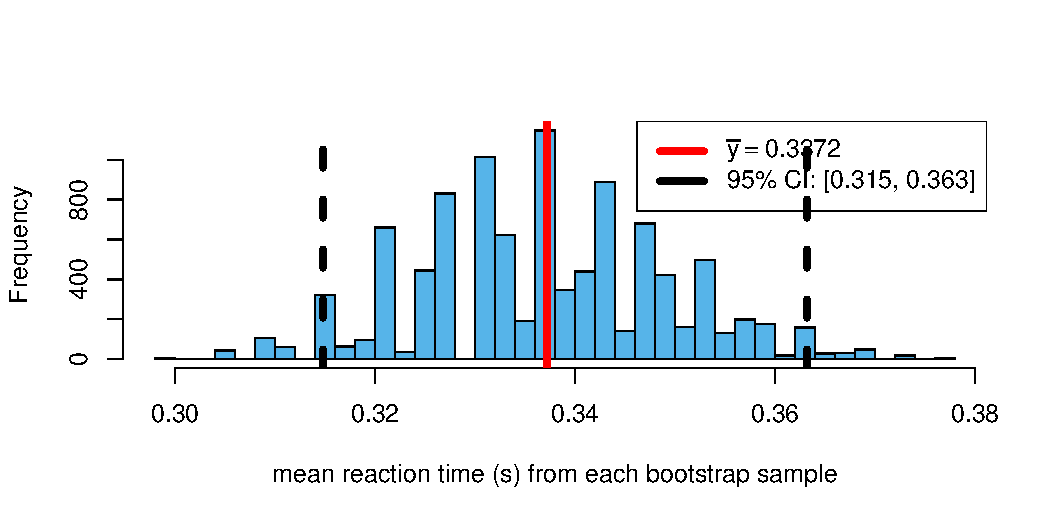
\includegraphics[width=\maxwidth]{figure/unnamed-chunk-36-1} 

}


\end{knitrout}
	
\end{frame}

%\section{One sample proportion}

%\begin{frame}
%	\begin{itemize}
%		\item Binomial calculations
%		\item Nomogram, Clopper-Pearson CI
%		\item Normal approximation
%	\end{itemize}
%\end{frame}


\section{p-values}

\begin{frame}
	\frametitle{$p$-values and statistical tests}
	
	
	%\vspace{18pt}
	\begin{definition}[$p$-value]
		A \textbf{probability concerning the observed data}, calculated under a \textbf{Null Hypothesis} assumption, i.e., assuming that the only factor operating is sampling or measurement variation. 
	\end{definition}
	
	\begin{itemize} 
		\item[\underline{Use}] To assess the evidence provided by the sample data
		in relation to a pre-specified claim or `hypothesis' concerning some parameter(s) or data-generating process. 
		\item[\underline{Basis}] As with a confidence interval, it makes use of the concept of a \textit{distribution}. 
		\item[\underline{Caution}] A $p$-value is NOT the probability that the null `hypothesis' is true
	\end{itemize}
\end{frame}


\begin{frame}
	\frametitle{More about the $p$-value}
	\small
	%\begin{footnotesize}
	\begin{itemize}
		\setlength\itemsep{.3em}
		\item The $p$-value is a \textbf{probability concerning data}, \textbf{conditional on the Null Hypothesis being true}. 
		\item \textbf{It is not the probability that Null Hypothesis is true}, \textit{conditional on the data.} 
		%\item Very few MDs mix up complement of specificity (i.e. probability of a `positive'  test result when in fact patient does not have disease in question) with positive predictive value (i.e. probability that a patient who has had a `positive'  test result does  have disease in question).
		\begin{align*}
			p_{value} & = P(\textrm{this or more extreme data}| H_0) \\
			& \neq P(H_0|\textrm{this or more extreme data}).
		\end{align*}
		
		
		\item Statistical tests are often coded as statistically significant or not according to whether results are extreme or not with respect to a reference (null)  distribution.  But a test result  is just one piece of data, and needs to be considered \textit{along with  rest of evidence} before coming to a `conclusion.' \item \textbf{Likewise with statistical `tests': the $p$-value is just one more piece of \textit{evidence}, hardly enough to `conclude' anything}. 
		%\item The probability that the DNA from the blood  of a randomly selected (innocent) person would match that from blood on crime-scene glove was 
		%$p=10^{-17}$. \textit{Do not equate this} Prob[data $|$ innocent] \textit{with its transpose}:
		%writing ``data'' as shorthand for ``this or more extreme data'', we need to be aware that 
		%$$p_{value} = Prob[ \ data \  | \  H_0 ] \neq Prob[ \ H_0 \  |  \ data ].$$
	\end{itemize}
	%\end{footnotesize}
\end{frame}

\begin{frame}
	\frametitle{The prosecutor's fallacy \footnote{\tiny{The Bayesian flip
				Correcting the prosecutor's fallacy. Significance. August 2015.}}}
	
	\begin{itemize}
		\setlength\itemsep{1em}
		\item Restating this both more succinctly, and in
		terms better suited to a statistically literate
		readership, the prosecutor’s fallacy is to
		calculate P(evidence | innocence) and interpret
		it as P(innocence | evidence). 
		\item It may be true
		that if the accused were innocent, there is only
		one chance in 3 million of a DNA match. But
		the DNA match does not necessarily imply
		that there is only one chance in 3 million
		of the accused being innocent. 
		\item Stated more
		generally, the prosecutor’s fallacy is
		$$P(A | B) = P(B | A)
		$$
		\item We know, from Bayes’ rule, that
		$$P(A | B) = \frac{P(B | A) P(A)}{P(B)}
		$$
	\end{itemize}
	
\end{frame}


\begin{frame}{The Bayesian Flip}
	
	\begin{itemize}
		\item In many investigations
		we may be presented with
		P(data | theory), but what
		we would really like to
		know is P(theory | data):
		the probability that our
		theory is correct, given what
		we have observed
		\item To move from P(data | theory) to
		P(theory | data), we need to do the Bayesian
		flip. 
		\item Every year in the United States 38 million
		women are tested for breast cancer with
		mammograms. Of these, 140 000 have cancer.
		Mammograms have been determined to be
		90\% accurate for women with breast cancer. 
		\item This figure was calculated by tallying all of
		the women who were eventually determined
		to have breast cancer and looking back to see
		if their initial mammograms were positive,
		thus: $$P(+mammogram | cancer) = 0.90$$
		and, using a similar empirical investigation,
		$$P(+mammogram | no cancer) = 0.10$$
	\end{itemize}
	
\end{frame}


\begin{frame}{The Bayesian Flip}
	
	\begin{itemize}
		\item It is important to know that
		a test is both powerful and has a relatively low
		rate of false positives. But when one is faced
		with a positive mammogram result, these are
		hardly useful. We administer a mammogram
		because we do not know whether or not
		someone has cancer.
		\item What we want to know is
		$$P(cancer | +mammogram)$$ \pause 
		\item This probability is a fraction
		that has as its numerator the number of
		women annually diagnosed with breast
		cancer via mammograms, or 140 000, and
		as its denominator the number of positive
		mammograms (including both true cancer
		cases and false positives):
		\begin{align*}
			P(cancer | +mammogram) &= \frac{True\, positives}{(True\,positives + False\, positives)} \\
			&= 140 000 / (140 000 + 0.1 × 38\,million)
			\\
			&= 140 000 / (140 000 + 3 800 000)
			\\
			&= 140 000 / 3 940 000 = 0.036 = 3.6\%
		\end{align*}
	\end{itemize}
	
\end{frame}




\begin{frame}
	\frametitle{Close relationship between $p$-value and CI}
	\begin{center}
		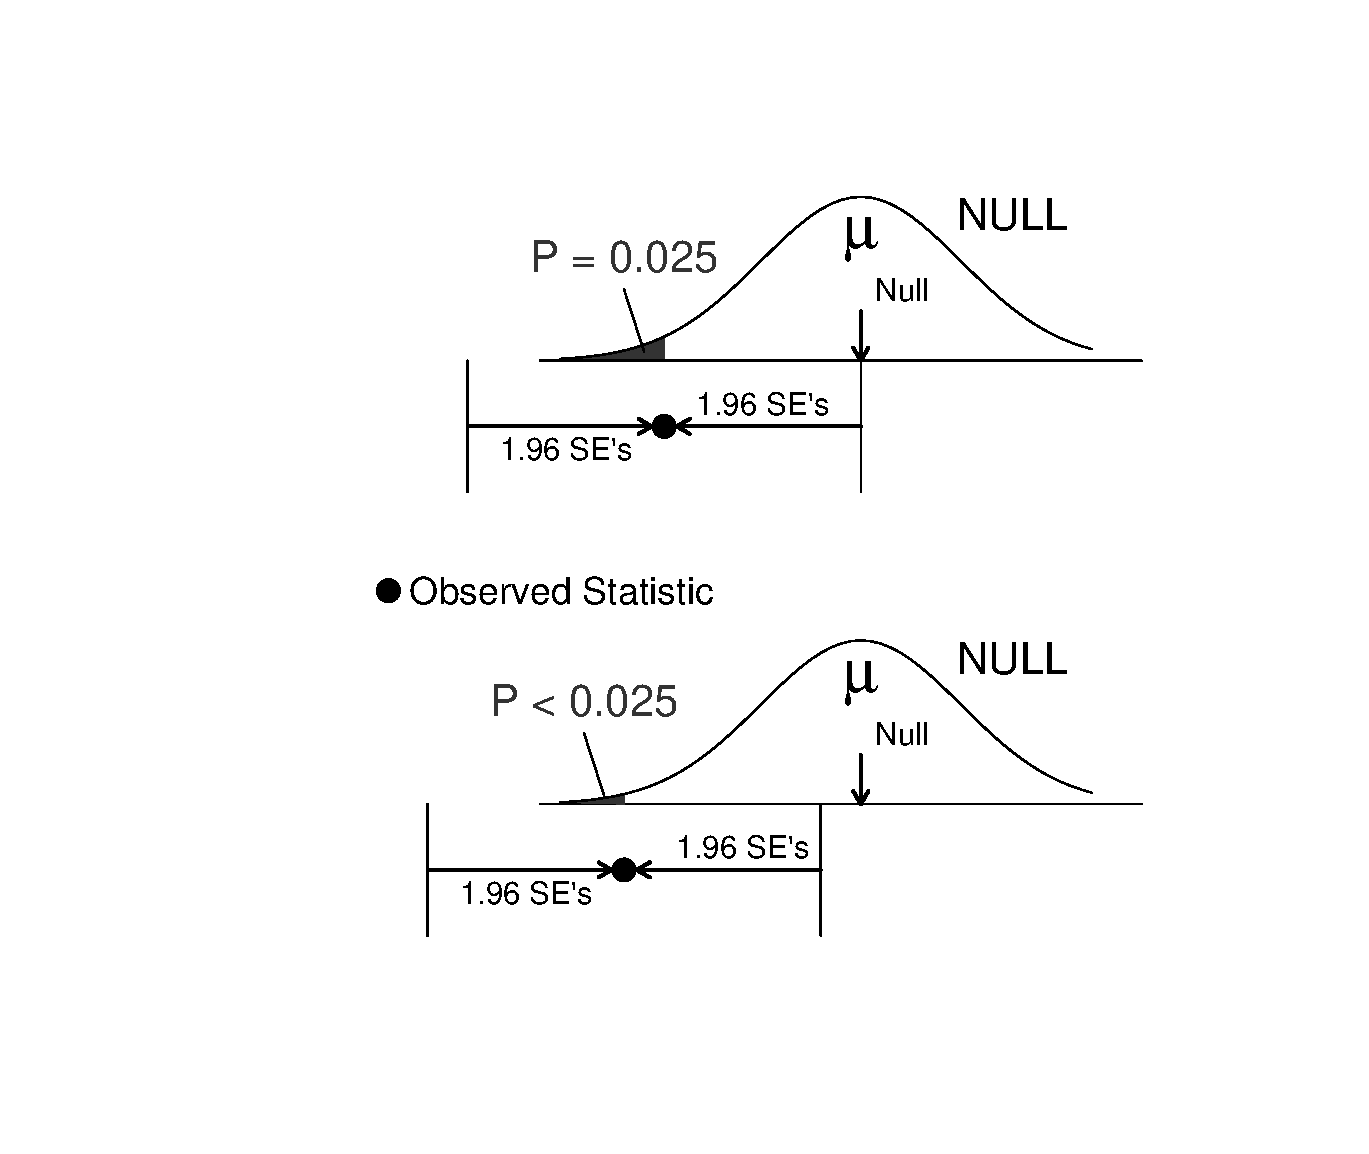
\includegraphics[width=1.65in]{P-CI.pdf}
	\end{center} 
	\begin{footnotesize}
		\begin{itemize}
			\item
			(Upper graph) If upper limit of 95\% CI\textit{ just touches} null value, then
			the 2 sided $p$-value is 0.05 (or 1 sided $p$-value is 0.025). 
			\item
			(Lower graph) If upper limit \textit{excludes} null value, then
			the 2 sided $p$-value is less than 0.05 (or 1 sided $p$-value is less than 0.025). 
			\item
			(Graph not shown) If  CI \textit{includes} null value, then the 2-sided $p$-value is greater than (the conventional) 0.05, and thus observed statistic is ``not statistically significantly different'' from hypothesized null value. 
		\end{itemize}
	\end{footnotesize}
\end{frame}




\section{Power and sample size}

\begin{frame}[fragile]{Power = $1 - \beta$}

\vspace*{-0.2in}

\begin{definition}[Power = $1-\beta$]
	The probability that a fixed level $\alpha$ significance test will reject $H_0$ when a particular alternative value of the parameter is true is called the \textbf{power} of the test to detect the alternative. 
\end{definition}


\vspace*{-0.08in}

\centering
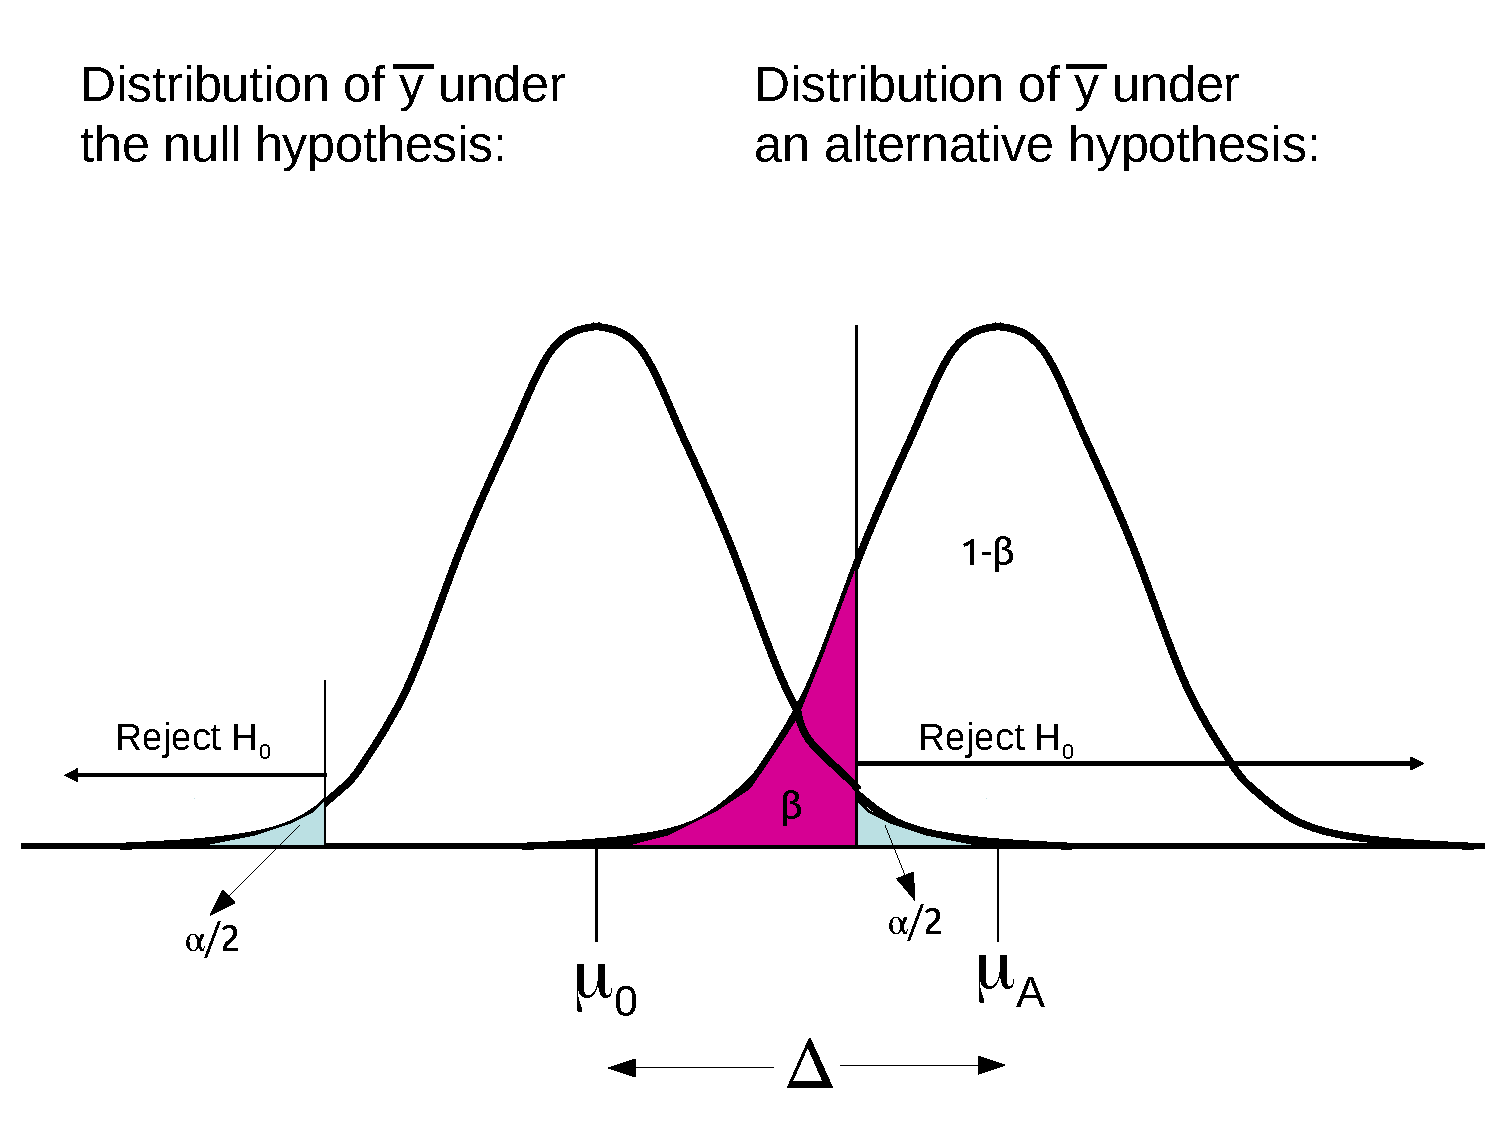
\includegraphics[scale=0.31]{HypTest3-3.pdf}


\end{frame}

\begin{frame}{Power and Sample Size: 3 questions}

\begin{enumerate}
	\setlength\itemsep{1em}
	\item How much water a supplier could add to the milk before they have a 10\% , 50\%, 80\%
	chance of getting caught, i.e., of the buyer detecting the cheating ? 
	\item Assume a 99:1 mix of milk and water. What are the chances of detecting cheating if the buyer uses samples $n$=10, 15 or 20 rather than just 5 measurements? 
	\item At what $n$ does the chance of detecting cheating reach 80\%? (\textit{a commonly used, but arbitrary, criterion used in sample-size planning by investigators seeking funding for their proposed research})
\end{enumerate}

\end{frame}


\begin{frame}[fragile]{If the supplier added 1\% water to the milk}
\begin{knitrout}\tiny
\definecolor{shadecolor}{rgb}{0.969, 0.969, 0.969}\color{fgcolor}

{\centering 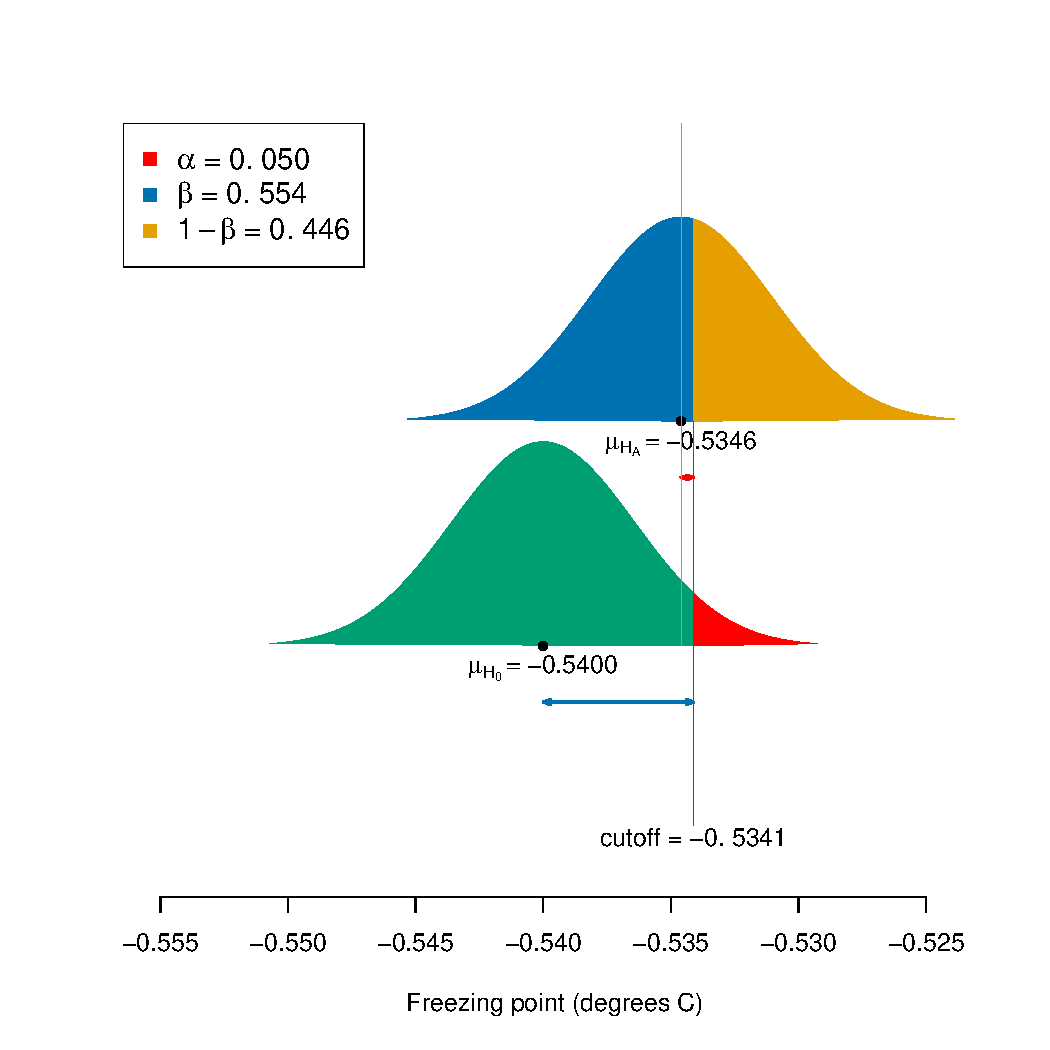
\includegraphics[width=\maxwidth]{figure/unnamed-chunk-37-1} 

}


\end{knitrout}
\end{frame}



\begin{frame}

\begin{center}
	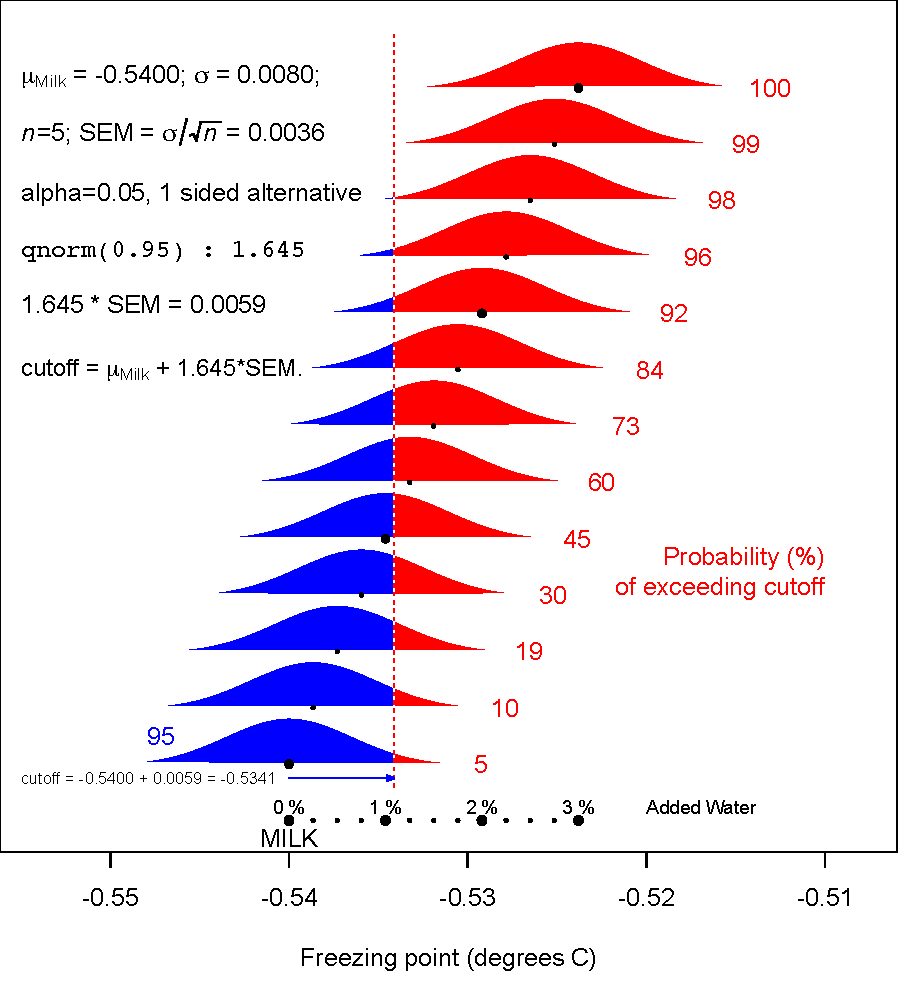
\includegraphics[scale=0.45]{ProbDetectingWaterInMilk.pdf} 
\end{center}

\vspace*{-0.18in}

{ \footnotesize
	The probabilities in red were calculated using the formula:
	\texttt{stats::pnorm(cutoff, mean = mu.mixture, sd = SEM, lower.tail=FALSE)}
}
\end{frame}



\begin{frame}[fragile]{The balancing formula}
\begin{knitrout}\tiny
\definecolor{shadecolor}{rgb}{0.969, 0.969, 0.969}\color{fgcolor}

{\centering 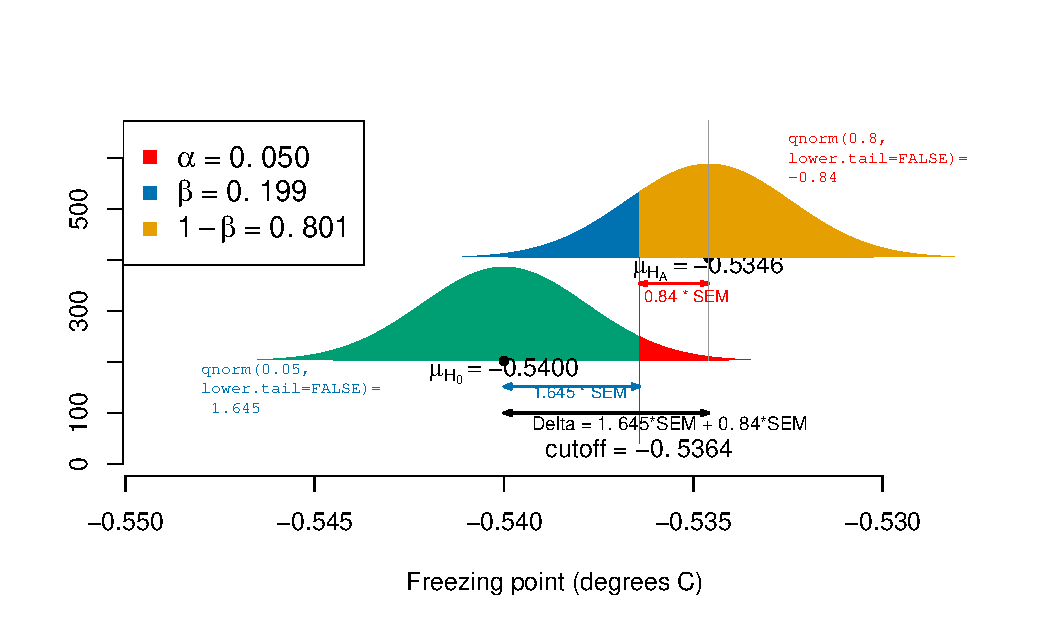
\includegraphics[width=\maxwidth]{figure/unnamed-chunk-38-1} 

}


\end{knitrout}
\end{frame}


\begin{frame}{What sample size needed?}

\begin{itemize}
	\setlength\itemsep{1em}
	\item The `balancing formula', in SEM terms, is simply the $n$ where
	$$ 1.645 \times SEM + 0.84 \times SEM = \Delta.$$
	Replacing each of the  SEMs (assumed equal, because we assumed the variability
	is approx. the same under both scenarios) by $\sigma/\sqrt{n}$,  i.e.,
	
	$$ 1.645 \times \sigma/\sqrt{n} + 0.84 \times \sigma/\sqrt{n} = \Delta.$$
	
	and solving for $n$, one gets
	
	$$  n = (1.645 + 0.84)^2  \times \bigg\{ \frac{\sigma}{\Delta} \bigg\}^2 = 
	(1.645 + 0.84)^2  \times \bigg\{ \frac{Noise}{Signal} \bigg\}^2 .$$
\end{itemize}

\end{frame}



\section{Part II}


\subsection{One Sample Rate}

\begin{frame}
	\frametitle{The Poisson Distribution}
	
	\begin{itemize}
		\small
		\setlength\itemsep{1em}
		\item The (infinite number of) probabilities $P_{0}, P_{1}, ..., P_{y}, ..., $ of observing 
		$Y = 0, 1, 2, \dots , y, \dots $ events in a given amount of ``experience.'' 
		
		\item These probabilities, $P(Y = k) \to$ \texttt{dpois()}, are governed by a single parameter, the mean $E[Y] = \mu$ which represents the expected \textbf{number} of events in the amount of experience actually studied. 
		
		\item We say that a random variable $Y \sim \textrm{Poisson}(\mu)$ distribution if 
		
		\[ P(Y=k) = \frac{\mu^k}{k!}e^{-\mu}, \quad k = 0, 1, 2, \ldots\]

		
		\item Note: in \texttt{dpois()} $\mu$ is referred to as \texttt{lambda}
		
		\item Note the distinction between $\mu$ and $\lambda$
		\begin{itemize}
			\item $\mu$: expected \textbf{number} of events
			\item $\lambda$: \textbf{rate} parameter
		\end{itemize}
	\end{itemize}
\end{frame}

\begin{frame}[fragile]{Confidence interval for $\mu$}
	\begin{itemize}
		\setlength\itemsep{2em}
		\item If the CLT hasn't kicked in, then the usual CI might not be appropriate: $$\textrm{point-estimate} \pm z^\star  \times \textrm{standard error}$$
		
		\pause 
		
		\item \texttt{qpois} function doesn't work either:
\begin{knitrout}\tiny
\definecolor{shadecolor}{rgb}{0.969, 0.969, 0.969}\color{fgcolor}\begin{kframe}
\begin{alltt}
\hlcom{# middle area is not 95%}
\hlstd{mosaic}\hlopt{::}\hlkwd{xqpois}\hlstd{(}\hlkwd{c}\hlstd{(}\hlnum{0.025}\hlstd{,} \hlnum{0.975}\hlstd{),} \hlkwc{lambda} \hlstd{=} \hlnum{6}\hlstd{)}
\end{alltt}
\end{kframe}

{\centering 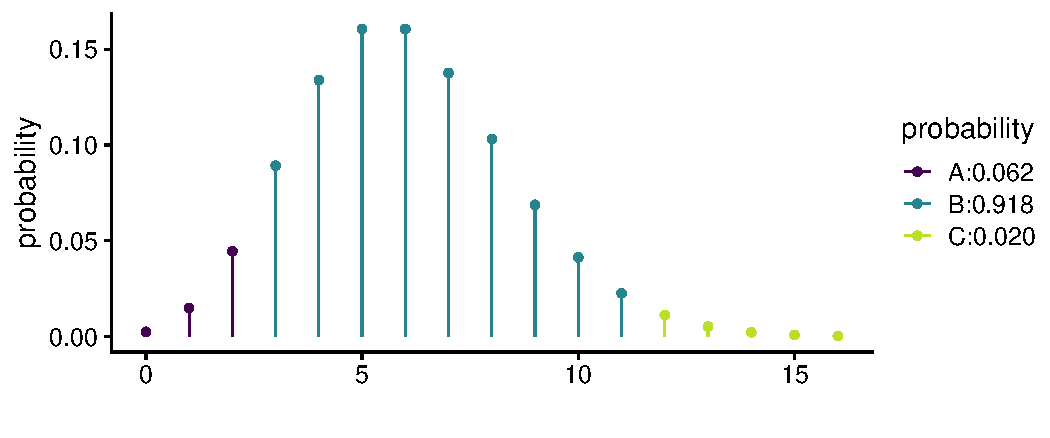
\includegraphics[width=\maxwidth]{figure/unnamed-chunk-39-1} 

}


\begin{kframe}\begin{verbatim}
## [1]  2 11
\end{verbatim}
\end{kframe}
\end{knitrout}
	\end{itemize}
\end{frame}





\begin{frame}[fragile]{Confidence interval for $\mu$}
	\begin{itemize}
		\setlength\itemsep{2em}
		
		\item Similar to the binomial (Clopper-Pearson CI), we consider a \textit{first-principles} $100(1-\alpha)\%$ CI $[\mu_{LOWER},\: \mu_{UPPER}]$ such that  
		$$P(Y \ge y \: | \: \mu_{LOWER}) = \alpha/2 \:\: \textrm{ and} \:\:  P(Y \le y \: | \: \mu_{UPPER}) = \alpha/2.$$
		\item For example, the  95\% CI for $\mu$, based on $y=6,$ is  $[\underline{2.20}, \underline{13.06}].$ 
		\item \textbf{Exercise:} can we use \texttt{glm} to get a CI for $\mu$ ?
	\end{itemize}
\end{frame}




\begin{frame}
	\centering
	\includegraphics[width=3in,height=4in]{CI_Poisson(6).pdf}
\end{frame}


\subsection{Regression}

\begin{frame}
	\Wider[8em]{
		\centering
		\includegraphics[width=4.9in,height=3.6in]{Fig16.pdf}
	}
\end{frame}

\subsubsection{Linear Regression}
\begin{frame}{Deterministic and stochastic model components}
	\begin{itemize}
		\item 
		The regression equation specifies the deterministic part of the model.
		
		\item This is defined in terms of parameters, conditional on the values of $X$.
		
		\item To complete the model specification, we need to specify the stochastic component of the model, a statistical distribution for the outcome $Y_{X}$. 
		\item The appropriate distribution is
		$$
		Y_{X} \sim \operatorname{Gaussian}\left(\mu_{X}, \sigma^2\right)
		$$
		\item Here the mean $\mu_{X}$ is given by the regression equation as 
		$$
		\mu_{X}=\mu_0 + \Delta_{\mu} \cdot X
		$$
	\end{itemize}
\end{frame}





\begin{frame}[fragile,plain]
	\vspace*{-0.3in}

	
\begin{knitrout}\tiny
\definecolor{shadecolor}{rgb}{0.969, 0.969, 0.969}\color{fgcolor}\begin{kframe}
\begin{alltt}
\hlstd{depths} \hlkwb{<-} \hlstd{readr}\hlopt{::}\hlkwd{read_csv}\hlstd{(}\hlstr{"depths.csv"}\hlstd{)}
\hlstd{fit} \hlkwb{<-} \hlkwd{lm}\hlstd{(alt} \hlopt{~} \hlnum{1}\hlstd{,} \hlkwc{data} \hlstd{= depths);} \hlkwd{print}\hlstd{(}\hlkwd{summary}\hlstd{(fit),} \hlkwc{signif.stars} \hlstd{= F)}
\end{alltt}
\begin{verbatim}
## Coefficients:
##             Estimate Std. Error t value Pr(>|t|)
## (Intercept)   3628.5       86.5      42   <2e-16
## 
## Residual standard error: 1730 on 399 degrees of freedom
\end{verbatim}
\begin{alltt}
\hlstd{fit} \hlkwb{<-} \hlkwd{lm}\hlstd{(alt} \hlopt{~} \hlstd{South,} \hlkwc{data} \hlstd{= depths);} \hlkwd{print}\hlstd{(}\hlkwd{summary}\hlstd{(fit),} \hlkwc{signif.stars} \hlstd{= F)}
\end{alltt}
\begin{verbatim}
## Coefficients:
##             Estimate Std. Error t value Pr(>|t|)
## (Intercept)     3523        122   28.82   <2e-16
## South            211        173    1.22     0.22
## 
## Residual standard error: 1730 on 398 degrees of freedom
## Multiple R-squared: 0.00372,	Adjusted R-squared: 0.00122 
## F-statistic: 1.49 on 1 and 398 DF,  p-value: 0.223
\end{verbatim}
\begin{alltt}
\hlstd{fit} \hlkwb{<-} \hlkwd{glm}\hlstd{(alt} \hlopt{~} \hlstd{South,} \hlkwc{data} \hlstd{= depths,} \hlkwc{family} \hlstd{=} \hlkwd{gaussian}\hlstd{(}\hlkwc{link}\hlstd{=log));} \hlkwd{print}\hlstd{(}\hlkwd{summary}\hlstd{(fit),} \hlkwc{signif.stars} \hlstd{= F)}
\end{alltt}
\begin{verbatim}
## 
## Coefficients:
##             Estimate Std. Error t value Pr(>|t|)
## (Intercept)   8.1671     0.0347  235.41   <2e-16
## South         0.0581     0.0477    1.22     0.22
## 
## (Dispersion parameter for gaussian family taken to be 2988040)
## 
##     Null deviance: 1193681102  on 399  degrees of freedom
## Residual deviance: 1189239546  on 398  degrees of freedom
## AIC: 7103
## 
## Number of Fisher Scoring iterations: 5
\end{verbatim}
\end{kframe}
\end{knitrout}
	
\end{frame}


\begin{frame}[fragile,plain]
	%\vspace*{-.0551in}
	%\scriptsize
	%	\textbf{2. Difference of mean depth in north vs south hemisphere}
	
	
\begin{knitrout}\tiny
\definecolor{shadecolor}{rgb}{0.969, 0.969, 0.969}\color{fgcolor}\begin{kframe}
\begin{alltt}
\hlkwd{coef}\hlstd{(fit)}
\end{alltt}
\begin{verbatim}
## (Intercept)       South 
##      8.1671      0.0581
\end{verbatim}
\begin{alltt}
\hlkwd{vcov}\hlstd{(fit)}
\end{alltt}
\begin{verbatim}
##             (Intercept)    South
## (Intercept)      0.0012 -0.00120
## South           -0.0012  0.00228
\end{verbatim}
\begin{alltt}
\hlkwd{confint}\hlstd{(fit)}
\end{alltt}
\begin{verbatim}
##               2.5 % 97.5 %
## (Intercept)  8.0967  8.233
## South       -0.0353  0.152
\end{verbatim}
\end{kframe}
\end{knitrout}
\end{frame}



\begin{frame}[fragile,plain]
	%	\vspace*{-0.2in}
	\small
	\textbf{2.2 Bootstrap CI for mean difference using canned function}
\begin{knitrout}\tiny
\definecolor{shadecolor}{rgb}{0.969, 0.969, 0.969}\color{fgcolor}\begin{kframe}
\begin{alltt}
\hlstd{pacman}\hlopt{::}\hlkwd{p_load}\hlstd{(car)}
\hlstd{betahat.boot} \hlkwb{<-} \hlstd{car}\hlopt{::}\hlkwd{Boot}\hlstd{(fit,} \hlkwc{R}\hlstd{=}\hlnum{999}\hlstd{)}
\hlkwd{head}\hlstd{(betahat.boot}\hlopt{$}\hlstd{t)}
\end{alltt}
\begin{verbatim}
##      (Intercept)  South
## [1,]        8.17 0.0713
## [2,]        8.14 0.0923
## [3,]        8.20 0.1109
## [4,]        8.18 0.0398
## [5,]        8.21 0.0135
## [6,]        8.13 0.1086
\end{verbatim}
\begin{alltt}
\hlkwd{dim}\hlstd{(betahat.boot}\hlopt{$}\hlstd{t)}
\end{alltt}
\begin{verbatim}
## [1] 999   2
\end{verbatim}
\begin{alltt}
\hlstd{deltamuhat.boot} \hlkwb{<-} \hlstd{betahat.boot}\hlopt{$}\hlstd{t[,}\hlnum{2}\hlstd{]}
\hlkwd{median}\hlstd{(deltamuhat.boot)}
\end{alltt}
\begin{verbatim}
## [1] 0.057
\end{verbatim}
\begin{alltt}
\hlkwd{quantile}\hlstd{(deltamuhat.boot,} \hlkwc{probs} \hlstd{=} \hlkwd{c}\hlstd{(}\hlnum{0.025}\hlstd{,} \hlnum{0.975}\hlstd{))}
\end{alltt}
\begin{verbatim}
##    2.5%   97.5% 
## -0.0373  0.1551
\end{verbatim}
\end{kframe}

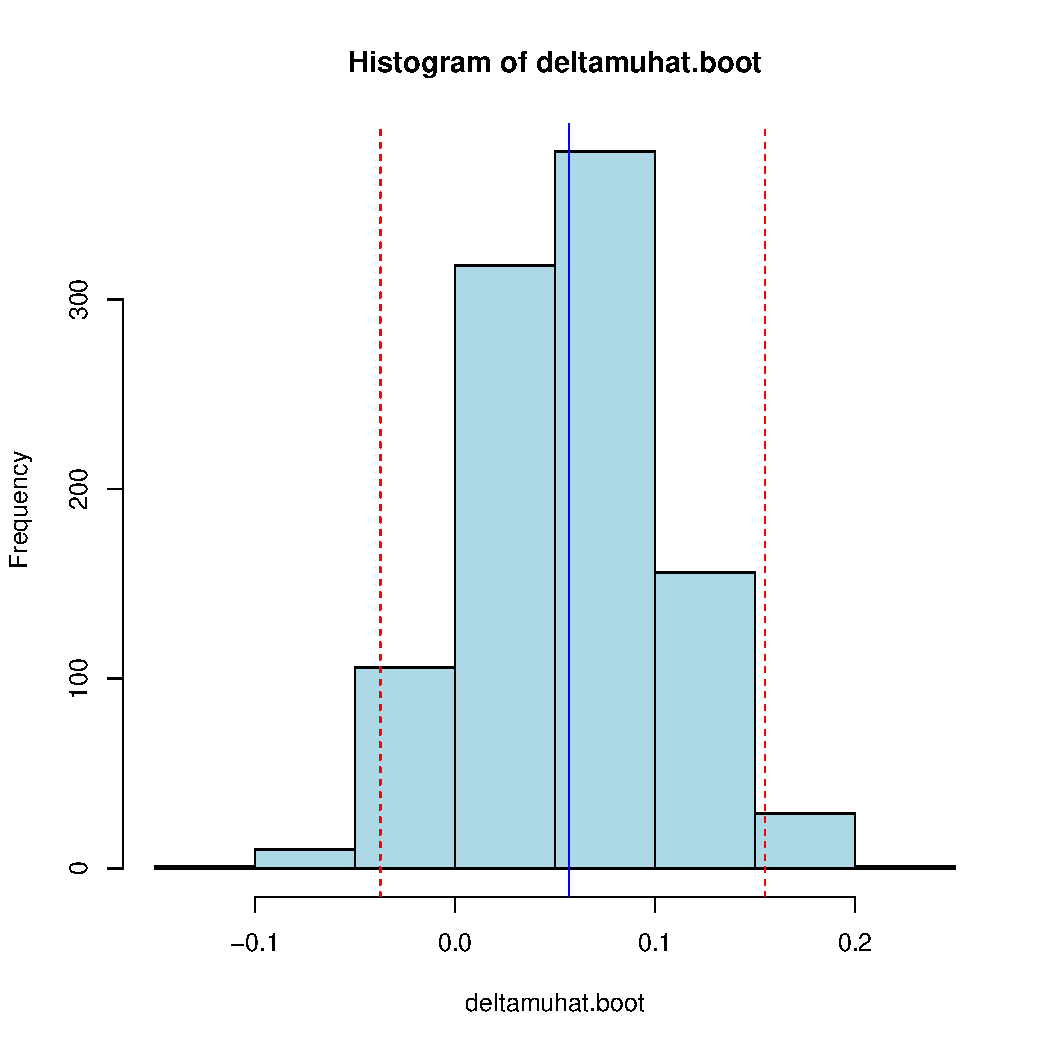
\includegraphics[width=0.35\textwidth]{figure/unnamed-chunk-42-1} \hfill{}


\end{knitrout}
	
\end{frame}


\begin{frame}[fragile,plain]
	%	\vspace*{-0.2in}
	\small
	\textbf{2.2 Bootstrap CI for mean difference using canned function (continued)}
\begin{knitrout}\tiny
\definecolor{shadecolor}{rgb}{0.969, 0.969, 0.969}\color{fgcolor}\begin{kframe}
\begin{alltt}
\hlkwd{summary}\hlstd{(betahat.boot)}
\end{alltt}
\begin{verbatim}
## 
## Number of bootstrap replications R = 999 
##             original  bootBias bootSE bootMed
## (Intercept)   8.1671  0.000348 0.0395   8.169
## South         0.0581 -0.000736 0.0490   0.057
\end{verbatim}
\begin{alltt}
\hlkwd{confint}\hlstd{(betahat.boot)}
\end{alltt}
\begin{verbatim}
## Bootstrap bca confidence intervals
## 
##              2.5 % 97.5 %
## (Intercept)  8.081  8.236
## South       -0.033  0.158
\end{verbatim}
\begin{alltt}
\hlkwd{hist}\hlstd{(betahat.boot)}
\end{alltt}
\end{kframe}

{\centering 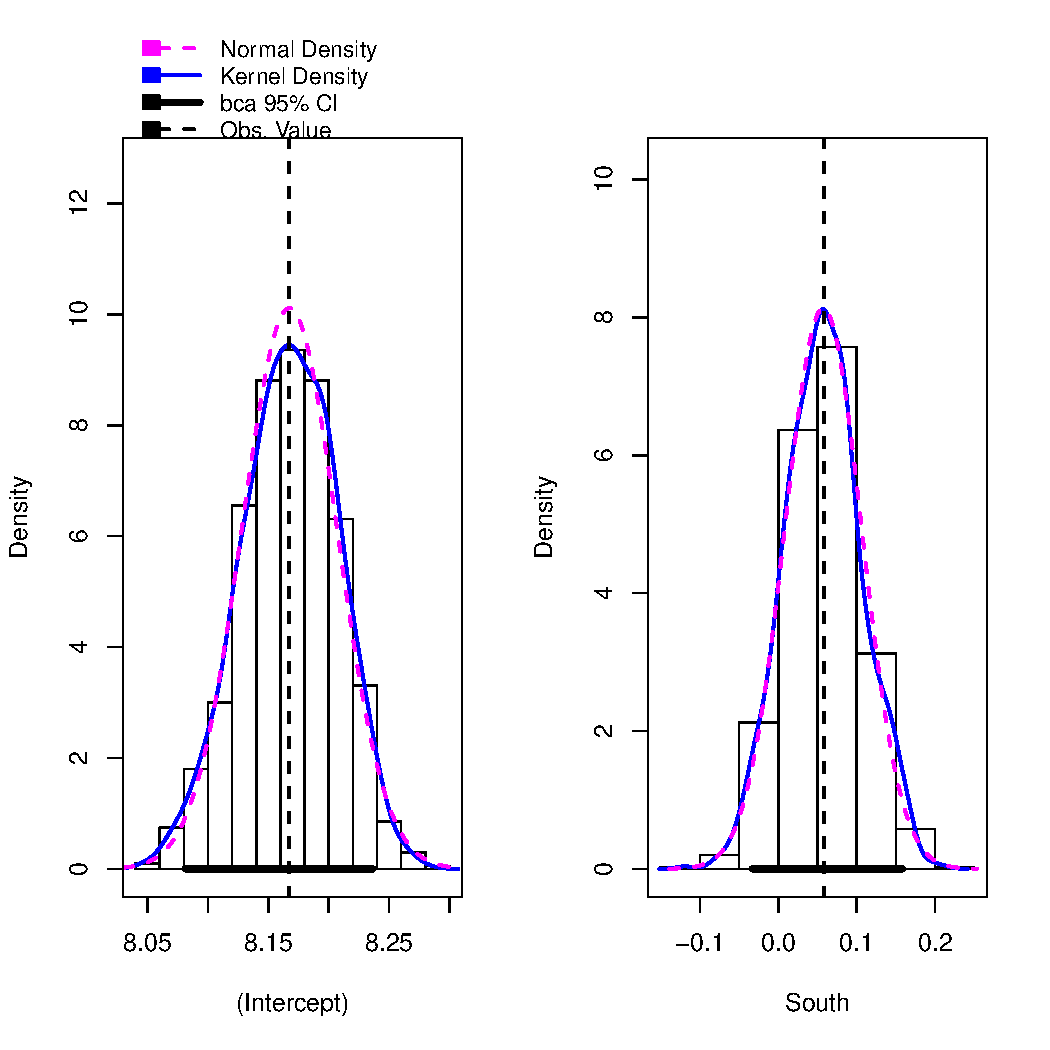
\includegraphics[width=0.55\textwidth]{figure/unnamed-chunk-43-1} 

}


\end{knitrout}
	
\end{frame}




\begin{frame}[fragile,plain]
	\textbf{2.3 Bootstrap CI for mean difference using \texttt{boot} package}
	\begin{figure}
		\begin{minipage}[h]{0.40\linewidth}
\begin{knitrout}\tiny
\definecolor{shadecolor}{rgb}{0.969, 0.969, 0.969}\color{fgcolor}\begin{kframe}
\begin{alltt}
\hlkwd{library}\hlstd{(boot)}
\hlcom{# function to obtain deltamu hat}
\hlstd{deltamu} \hlkwb{<-} \hlkwa{function}\hlstd{(}\hlkwc{data}\hlstd{,} \hlkwc{indices}\hlstd{) \{}
\hlcom{# allows boot to select sample}
\hlstd{d} \hlkwb{<-} \hlstd{data[indices,]}
\hlstd{fit} \hlkwb{<-} \hlkwd{lm}\hlstd{(alt} \hlopt{~} \hlstd{South,} \hlkwc{data}\hlstd{=d)}
\hlkwd{coef}\hlstd{(fit)[}\hlstr{"South"}\hlstd{]}
\hlstd{\}}

\hlstd{results} \hlkwb{<-} \hlstd{boot}\hlopt{::}\hlkwd{boot}\hlstd{(}\hlkwc{data} \hlstd{= depths,}
\hlkwc{statistic} \hlstd{= deltamu,} \hlkwc{R}\hlstd{=}\hlnum{999}\hlstd{)}

\hlstd{results}
\end{alltt}
\begin{verbatim}
## 
## ORDINARY NONPARAMETRIC BOOTSTRAP
## 
## 
## Call:
## boot::boot(data = depths, statistic = deltamu, R = 999)
## 
## 
## Bootstrap Statistics :
##     original  bias    std. error
## t1*      211   -7.25         172
\end{verbatim}
\end{kframe}
\end{knitrout}
			
		\end{minipage}
		\hspace{0.4cm}
		\begin{minipage}[h]{0.50\linewidth}
\begin{knitrout}\tiny
\definecolor{shadecolor}{rgb}{0.969, 0.969, 0.969}\color{fgcolor}\begin{kframe}
\begin{alltt}
\hlkwd{plot}\hlstd{(results)}
\end{alltt}
\end{kframe}

{\centering 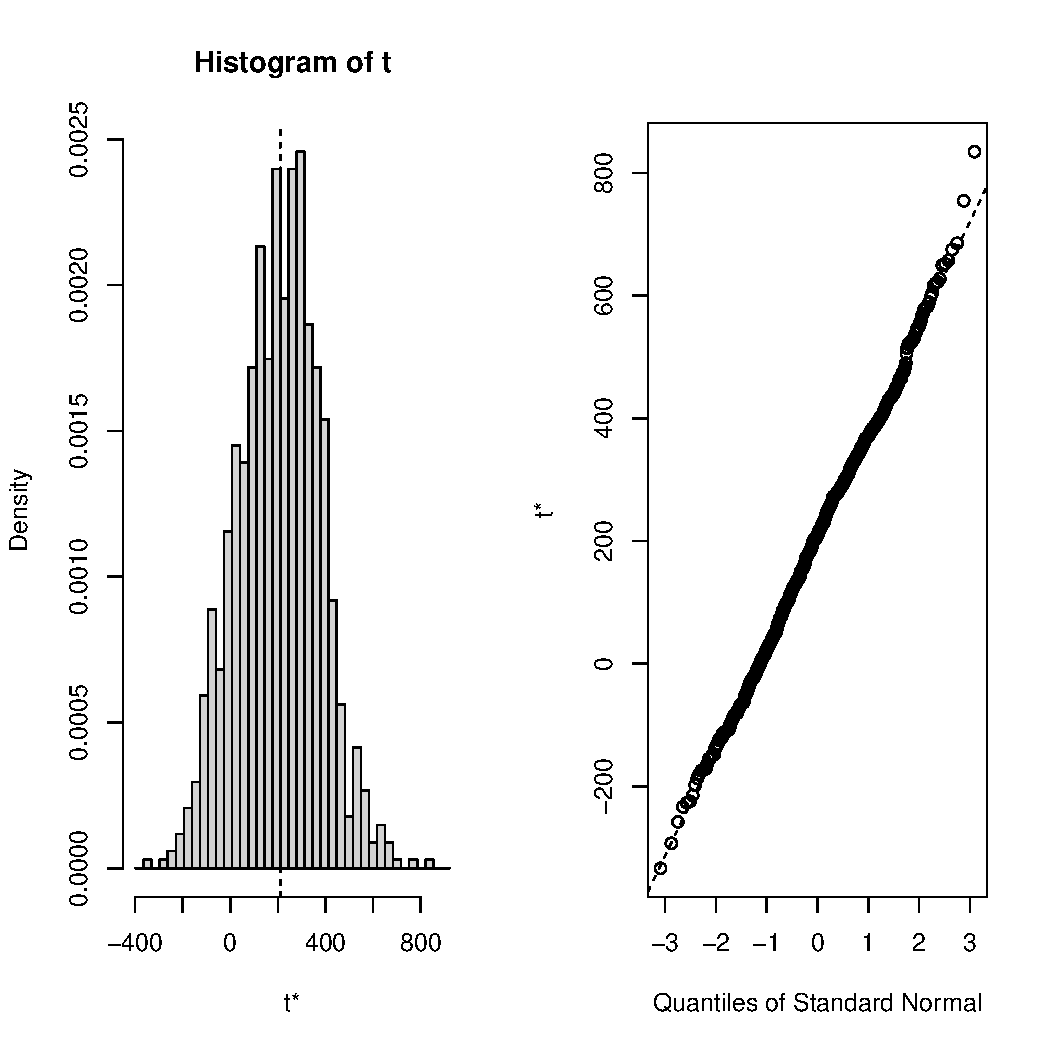
\includegraphics[width=\maxwidth]{figure/unnamed-chunk-45-1} 

}


\begin{kframe}\begin{alltt}
\hlkwd{boot.ci}\hlstd{(results)}
\end{alltt}
\begin{verbatim}
## BOOTSTRAP CONFIDENCE INTERVAL CALCULATIONS
## Based on 999 bootstrap replicates
## 
## CALL : 
## boot.ci(boot.out = results)
## 
## Intervals : 
## Level      Normal              Basic         
## 95%   (-119,  555 )   (-125,  552 )  
## 
## Level     Percentile            BCa          
## 95%   (-130,  546 )   (-123,  548 )  
## Calculations and Intervals on Original Scale
\end{verbatim}
\end{kframe}
\end{knitrout}
		\end{minipage}
	\end{figure}
\end{frame}


\begin{frame}{Permutation Testing}
	\begin{itemize}
		\item In testing a null hypothesis we need a test statistic that will have different values under the null hypothesis and the alternatives we	care about 
		\item We then need to compute the sampling distribution of the test	statistic when the null hypothesis is true. For some test statistics	and some null hypotheses this can be done analytically. 
		\item The pvalue is the probability that the test statistic would be at	least as extreme as we observed, if the null hypothesis is true.
		\item A permutation test gives a simple way to compute the sampling	distribution for any test statistic, under the null hypothesis that there is no effect (i.e. South is not a determinant of the mean depth of the ocean)
		\item \url{https://www.jwilber.me/permutationtest/}
	\end{itemize}
\end{frame}


\begin{frame}{Permutation Testing}
	\begin{itemize}
		\item To estimate the sampling distribution of the test statistic we
		need many samples generated under the strong null hypothesis.
		\item If the null hypothesis is true, changing the exposure would have
		no effect on the outcome. By randomly shuffling the determinants
		we can make up as many data sets as we like.
		\item If the null hypothesis is true, the shuffled data sets should look
		like the real data, otherwise they should look different from the real data.
		\item The ranking of the real test statistic among the shuffled test
		statistics gives a p-value
	\end{itemize}
\end{frame}


\begin{frame}[fragile]{Permutation Testing}
\begin{knitrout}\tiny
\definecolor{shadecolor}{rgb}{0.969, 0.969, 0.969}\color{fgcolor}\begin{kframe}
\begin{alltt}
\hlstd{one.test} \hlkwb{<-} \hlkwa{function}\hlstd{(}\hlkwc{x}\hlstd{,}\hlkwc{y}\hlstd{) \{}
\hlstd{xstar} \hlkwb{<-} \hlkwd{sample}\hlstd{(x)}
\hlkwd{mean}\hlstd{(y[xstar}\hlopt{==}\hlnum{1}\hlstd{])} \hlopt{-} \hlkwd{mean}\hlstd{(y[xstar}\hlopt{==}\hlnum{0}\hlstd{])}
\hlstd{\}}

\hlstd{null.dist} \hlkwb{<-} \hlkwd{replicate}\hlstd{(}\hlnum{1000}\hlstd{,} \hlkwd{one.test}\hlstd{(}\hlkwc{x} \hlstd{= depths}\hlopt{$}\hlstd{South,} \hlkwc{y} \hlstd{= depths}\hlopt{$}\hlstd{alt))}
\hlkwd{hist}\hlstd{(null.dist)}
\hlkwd{abline}\hlstd{(}\hlkwc{v}\hlstd{=}\hlkwd{coef}\hlstd{(fit)[}\hlstr{"South"}\hlstd{],} \hlkwc{lwd}\hlstd{=}\hlnum{2}\hlstd{,} \hlkwc{col}\hlstd{=}\hlstr{"blue"}\hlstd{)}
\end{alltt}
\end{kframe}

{\centering 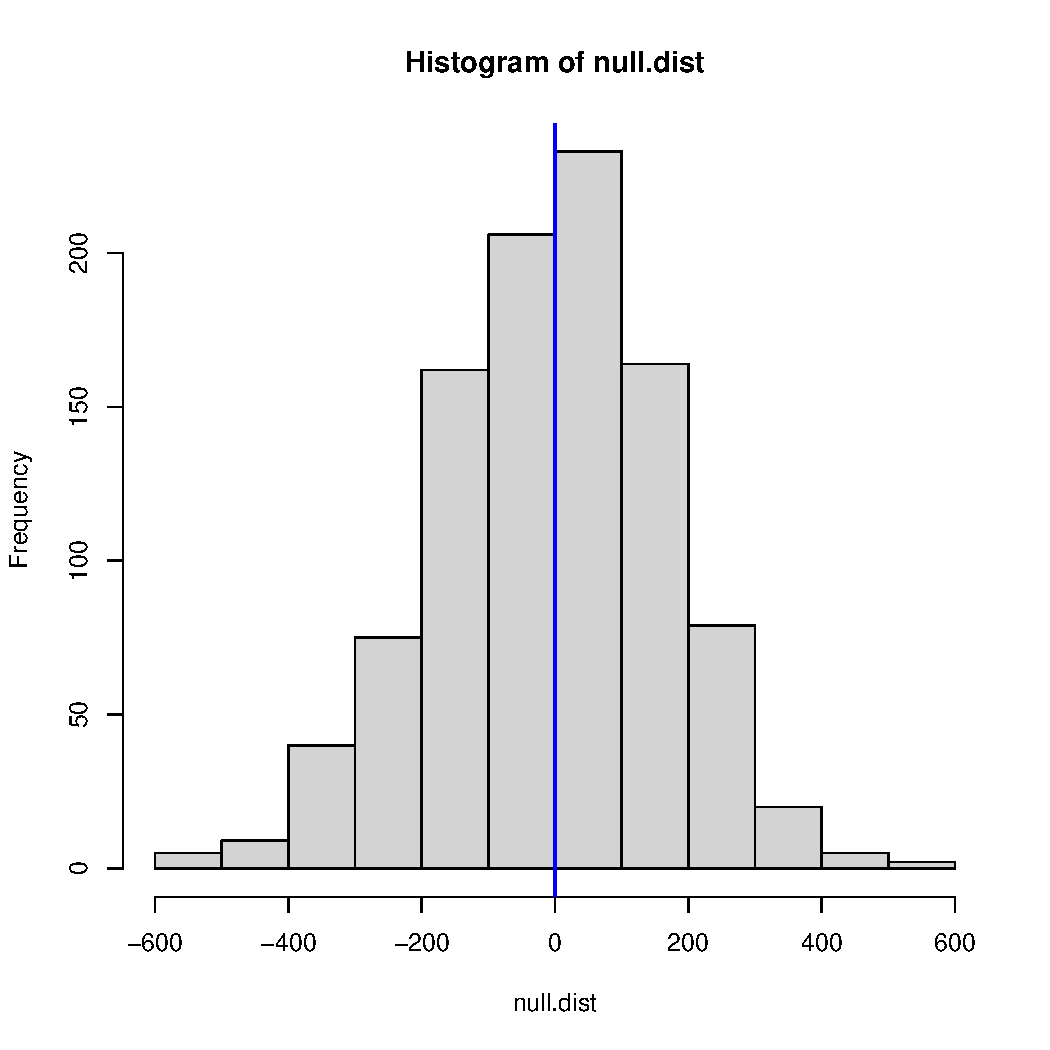
\includegraphics[width=0.5\textwidth]{figure/unnamed-chunk-46-1} 

}


\begin{kframe}\begin{alltt}
\hlkwd{mean}\hlstd{(}\hlkwd{abs}\hlstd{(null.dist)} \hlopt{>} \hlkwd{abs}\hlstd{(}\hlkwd{coef}\hlstd{(fit)[}\hlstr{"South"}\hlstd{]))}
\end{alltt}
\begin{verbatim}
## [1] 1
\end{verbatim}
\end{kframe}
\end{knitrout}
\end{frame}



\subsubsection{Poisson Regression}
\begin{frame}{Deterministic and stochastic model components}
	\begin{itemize}
		\item 
		The regression equation specifies the deterministic part of the model.
		
		\item This is defined in terms of parameters, conditional on the values of $X$.
		
		\item To complete the model specification, we need to specify the stochastic component of the model, a statistical distribution for the outcome $Y_{X}$ (counts). 
		\item The appropriate distribution is
		$$
		Y_{X} \sim \operatorname{Poisson}\left(\mu_{X}\right)
		$$
		\item Here the mean $\mu_{X}$ is given by the regression equation as 
		$$
		\mu_{X}=\lambda \cdot \textrm{PT}
		$$
	\end{itemize}
\end{frame}

\begin{frame}[fragile,plain]
	\vspace*{-1.091in}
	\tiny
	See the 2018 Lancet article \textit{Efficacy of Olyset Duo, a bednet containing pyriproxyfen and permethrin, versus a permethrin-only net against clinical malaria in an area with highly pyrethroid-resistant vectors in rural Burkina Faso: a cluster-randomised controlled trial} by Tiono et. al. Reproduce the Rate ratio (95\% CI) in Table 2. Calculate the rate difference and 95\% CI comparing PPF-treated to Standard long-lasting insecticidal nets. Check the goodness of fit. 
	

	
	
\begin{knitrout}\tiny
\definecolor{shadecolor}{rgb}{0.969, 0.969, 0.969}\color{fgcolor}\begin{kframe}
\begin{verbatim}
## Call:
## glm(formula = cases ~ exposure + offset(log(years)), family = poisson(link = log), 
##     data = df)
## 
## Coefficients:
##             Estimate Std. Error z value Pr(>|z|)
## (Intercept)   0.6831     0.0243   28.09  < 2e-16
## exposure     -0.2669     0.0329   -8.12  4.6e-16
## 
## (Dispersion parameter for poisson family taken to be 1)
## 
##     Null deviance: 1381.2  on 23  degrees of freedom
## Residual deviance: 1316.0  on 22  degrees of freedom
## AIC: 1477
## 
## Number of Fisher Scoring iterations: 5
\end{verbatim}
\end{kframe}
\end{knitrout}
	
\end{frame}


\subsubsection{Logistic Regression}

\begin{frame}{Deterministic and stochastic model components}
	\begin{itemize}
		\item 
		The regression equation specifies the deterministic part of the model.
		
		\item This is defined in terms of parameters, conditional on the values of $Z$ and $X$.
		
		\item To complete the model specification, we need to specify the stochastic component of the model, a statistical distribution for the outcome $D_{Z X}$. 
		\item It is already obvious that the appropriate distribution is
		$$
		D_{Z X} \sim \operatorname{Binomial}\left(N_{Z X}, \pi_{Z X}\right)
		$$
		\item Here the risk $\pi_{Z X}$ is given by the regression equation as (verify)
		$$
		\pi_{Z X}=\frac{e^{\alpha+\beta Z+\gamma X}}{1+e^{\alpha+\beta Z+\gamma X}}=\frac{1}{1+e^{-(\alpha+\beta Z+\gamma X)}}
		$$
		\item This inverse transformation is the so-called \textit{expit} function:
		$$
		\pi_{Z X}=\operatorname{logit}^{-1}(\alpha+\beta Z+\gamma X)=\operatorname{expit}(\alpha+\beta Z+\gamma X)
		$$
	\end{itemize}
\end{frame}

\begin{frame}{Regression equation with logit link}
	\begin{itemize}
		\item Reparametrizing the log-odds is referred to as logistic regression.
		\item In the ongoing example we may take
		$$
		\log \left(\frac{\pi_{Z X}}{1-\pi_{Z X}}\right)=\alpha+\beta Z+\gamma X
		$$
		\item The original four parameters are now expressed in terms of three new parameters: an intercept term $\alpha$ and regression coefficients $\beta$ and $\gamma$.
		\item The function $\log \frac{\pi}{1-\pi}$ is referred to as the logit transformation of the risk parameter $\pi$.
		\item Thus, the same model can be specified as a reparametrization of the risk parameter together with the \textit{logit link} function:
		$$
		\operatorname{logit}\left(\pi_{Z X}\right)=\alpha+\beta Z+\gamma X
		$$
	\end{itemize}
\end{frame}

\begin{frame}[fragile]{Log-linear model for risk}
	\begin{itemize}
		\item Is there some particular reason why we \textit{have} to use the logit link when modeling risk?
		\item Why could we not just parametrize the log-risk as
		$$
		\log(\pi_{ZX}) = \alpha + \beta Z + \gamma X ?
		$$
		\item We can; in this case the regression coefficient $\beta$ would be interpreted as a log-risk ratio:
		$$\begin{aligned}
		\frac{\pi_{1 X}}{\pi_{0 X}} &=\frac{e^{\alpha+\beta+\gamma X}}{e^{\alpha+\gamma X}} \\
		&=\frac{e^{\alpha} e^{\beta} e^{\gamma X}}{e^{\alpha} e^{\gamma X}} \\
		&=e^{\beta} \\
		\Leftrightarrow \log \left(\frac{\pi_{1 X}}{\pi_{0 X}}\right) &=\beta
		\end{aligned}$$
	\end{itemize}
\end{frame}

\section{ROC Curves}

\begin{frame}[fragile]{ROC Curves}
\begin{knitrout}\tiny
\definecolor{shadecolor}{rgb}{0.969, 0.969, 0.969}\color{fgcolor}\begin{kframe}
\begin{alltt}
\hlstd{fit1} \hlkwb{<-} \hlkwd{glm}\hlstd{(sta} \hlopt{~} \hlstd{type,} \hlkwc{family}\hlstd{=}\hlkwd{binomial}\hlstd{(}\hlkwc{link}\hlstd{=logit),} \hlkwc{data}\hlstd{=icu)}
\hlstd{fit2} \hlkwb{<-} \hlkwd{glm}\hlstd{(sta} \hlopt{~} \hlstd{type} \hlopt{+} \hlstd{age,} \hlkwc{family}\hlstd{=}\hlkwd{binomial}\hlstd{(}\hlkwc{link}\hlstd{=logit),} \hlkwc{data}\hlstd{=icu)}
\end{alltt}
\end{kframe}

{\centering 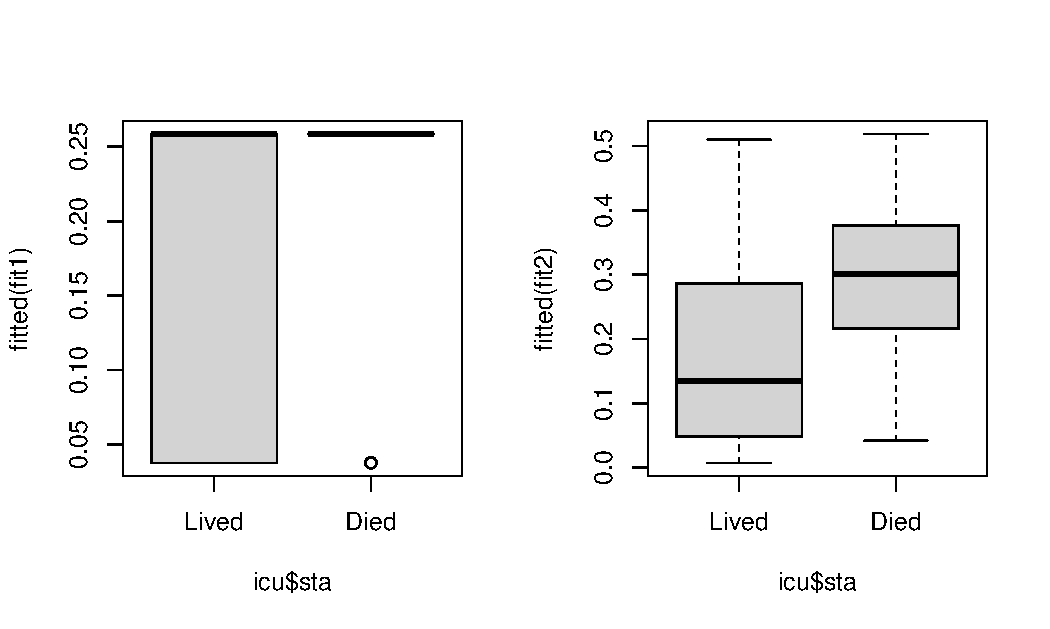
\includegraphics[width=\maxwidth]{figure/unnamed-chunk-49-1} 

}


\end{knitrout}
\end{frame}


\begin{frame}[fragile]{ROC Curves}
\begin{knitrout}\tiny
\definecolor{shadecolor}{rgb}{0.969, 0.969, 0.969}\color{fgcolor}

{\centering 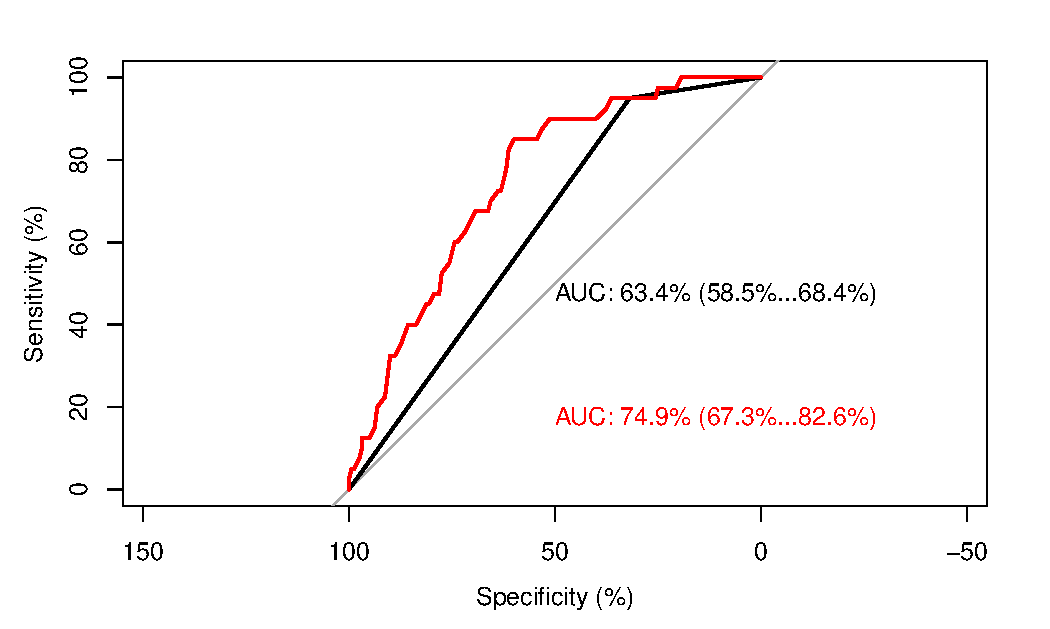
\includegraphics[width=\maxwidth]{figure/unnamed-chunk-50-1} 

}


\end{knitrout}
\end{frame}


\begin{frame}[fragile]{Session Info}
	\tiny
	
\begin{knitrout}\tiny
\definecolor{shadecolor}{rgb}{0.969, 0.969, 0.969}\color{fgcolor}\begin{kframe}
\begin{verbatim}
R version 4.1.1 (2021-08-10)
Platform: x86_64-pc-linux-gnu (64-bit)
Running under: Pop!_OS 21.04

Matrix products: default
BLAS:   /usr/lib/x86_64-linux-gnu/openblas-pthread/libblas.so.3
LAPACK: /usr/lib/x86_64-linux-gnu/openblas-pthread/libopenblasp-r0.3.13.so

attached base packages:
[1] tools     stats     graphics  grDevices utils     datasets  methods  
[8] base     

other attached packages:
 [1] pROC_1.16.2        boot_1.3-27        car_3.0-9          carData_3.0-4     
 [5] latex2exp_0.4.0    RColorBrewer_1.1-2 colorspace_2.0-2   oibiostat_0.2.0   
 [9] DT_0.16            mosaic_1.7.0       Matrix_1.3-2       mosaicData_0.20.1 
[13] ggformula_0.9.4    ggstance_0.3.4     lattice_0.20-41    kableExtra_1.2.1  
[17] socviz_1.2         gapminder_0.3.0    here_0.1           NCStats_0.4.7     
[21] FSA_0.8.30         forcats_0.5.1      stringr_1.4.0      dplyr_1.0.7       
[25] purrr_0.3.4        readr_1.4.0        tidyr_1.1.4        tibble_3.1.5      
[29] ggplot2_3.3.5.9000 tidyverse_1.3.0    knitr_1.36        

loaded via a namespace (and not attached):
  [1] readxl_1.3.1       backports_1.2.1    plyr_1.8.6        
  [4] splines_4.1.1      crosstalk_1.1.1    leaflet_2.0.3     
  [7] TH.data_1.0-10     digest_0.6.28      htmltools_0.5.2   
 [10] fansi_0.5.0        magrittr_2.0.1     mosaicCore_0.8.0  
 [13] openxlsx_4.1.5     modelr_0.1.8       sandwich_2.5-1    
 [16] blob_1.2.1         rvest_1.0.0        ggrepel_0.9.1.9999
 [19] haven_2.3.1        xfun_0.26          crayon_1.4.1      
 [22] jsonlite_1.7.2     lme4_1.1-23        survival_3.2-13   
 [25] zoo_1.8-8          glue_1.4.2         polyclip_1.10-0   
 [28] gtable_0.3.0       emmeans_1.5.1      webshot_0.5.2     
 [31] sjstats_0.18.0     sjmisc_2.8.5       abind_1.4-5       
 [34] scales_1.1.1       mvtnorm_1.1-1      DBI_1.1.1         
 [37] rstatix_0.6.0      ggeffects_0.16.0   Rcpp_1.0.7        
 [40] viridisLite_0.4.0  xtable_1.8-4       performance_0.8.0 
 [43] foreign_0.8-81     datawizard_0.2.1   htmlwidgets_1.5.3 
 [46] httr_1.4.2         ellipsis_0.3.2     pkgconfig_2.0.3   
 [49] farver_2.1.0       dbplyr_1.4.4       utf8_1.2.2        
 [52] tidyselect_1.1.1   labeling_0.4.2     rlang_0.4.12      
 [55] effectsize_0.5     munsell_0.5.0      TeachingDemos_2.12
 [58] cellranger_1.1.0   cli_3.0.1          generics_0.1.0    
 [61] pacman_0.5.1       sjlabelled_1.1.7   broom_0.7.9       
 [64] evaluate_0.14      fastmap_1.1.0      ggdendro_0.1.22   
 [67] fs_1.5.0           zip_2.2.0          nlme_3.1-152      
 [70] xml2_1.3.2         compiler_4.1.1     rstudioapi_0.13   
 [73] curl_4.3.2         ggsignif_0.6.3     reprex_0.3.0      
 [76] statmod_1.4.34     tweenr_1.0.1       stringi_1.7.5     
 [79] highr_0.9          parameters_0.15.0  nloptr_1.2.2.2    
 [82] vctrs_0.3.8        pillar_1.6.4       lifecycle_1.0.1   
 [85] estimability_1.3   data.table_1.14.2  cowplot_1.1.0     
 [88] insight_0.14.5     R6_2.5.1           gridExtra_2.3     
 [91] rio_0.5.16         codetools_0.2-18   MASS_7.3-53.1     
 [94] assertthat_0.2.1   rprojroot_2.0.2    withr_2.4.2       
 [97] multcomp_1.4-13    bayestestR_0.11.0  hms_1.1.1         
[100] grid_4.1.1         sjPlot_2.8.9       coda_0.19-4       
[103] minqa_1.2.4        rmarkdown_2.11.3   snakecase_0.11.0  
[106] ggpubr_0.4.0       ggforce_0.3.2      lubridate_1.8.0   
\end{verbatim}
\end{kframe}
\end{knitrout}
	
\end{frame}

\end{document}
